\documentclass[11pt,a4paper]{article}

% ── Packages ─────────────────────────────────────────────────────────
\usepackage[utf8]{inputenc}
\usepackage[T1]{fontenc}
\usepackage[margin=2.5cm]{geometry}
\usepackage{graphicx}
\usepackage{booktabs}
\usepackage{hyperref}
\usepackage[numbers,sort&compress]{natbib}
\usepackage{amsmath}
\usepackage{xcolor}
\usepackage{float}
\usepackage{caption}
\usepackage{subcaption}
\usepackage{tabularx}
\usepackage{multirow}
\usepackage{setspace}
\usepackage{lineno}

% siunitx-lite: format numbers without the full siunitx package
\newcommand{\num}[1]{\ensuremath{\mathrm{#1}}}

\graphicspath{{fig/}}

\hypersetup{
    colorlinks=true,
    linkcolor=blue!60!black,
    citecolor=green!50!black,
    urlcolor=blue!70!black,
}

\onehalfspacing
\linenumbers

% ── Title ─────────────────────────────────────────────────────────────
\title{%
  \textbf{Plant Science is Reorganizing Around Climate-Relevant Crops:\\
  Evidence from 4.9 Million Publications}
}

\author{%
  Ehsan Estaji\textsuperscript{1},
  Jian-Feng Mao\textsuperscript{1,*}
  \\[0.5em]
  \small \textsuperscript{1}Ume\aa\ Plant Science Centre (UPSC), Department of
         Plant Physiology, Ume\aa\ University, Ume\aa, Sweden \\[0.3em]
  \small \textsuperscript{*}Corresponding author: \texttt{jianfeng.mao@umu.se}
  \\[0.2em]
  \small ORCID: E.E.\ 0009-0005-0838-228X;\ \ J.-F.M.\ 0000-0001-9735-8516
}

\date{}

\begin{document}
\maketitle

% ── Abstract ─────────────────────────────────────────────────────────
\begin{abstract}
Whether plant science is pivoting toward climate-resilient crops
remains an open empirical question. Analysing \num{4.9} million
publications (1900--2024) from OpenAlex and PubMed, we find that
annual output over the modern era (1990--2024) follows a logistic
trajectory ($K = 217{,}781$ papers/year, inflection 2006), ending
exponential expansion. \textit{Arabidopsis thaliana}'s share has declined since
2012 while rice, wheat, and maize have risen; 40 sleeping-beauty
papers on minor crops awoke in 2019--2022; CRISPR reached mainstream
adoption twice as fast as prior genomic tools. A persistent
orphan-crop attention gap shows the realignment is incomplete. A
temporal placebo against a 1970--1999 null window (permutation
$p = 0.001$) confirms the shift is era-specific. Citation-flow
analysis reframes the \textit{Arabidopsis} decline as consolidation:
the crop-paper citation share to \textit{Arabidopsis} grew nine-fold
(1995--2016) and the reverse-translation lag collapsed from 6.5 to
2 years.
\textit{Arabidopsis} has become crop science's foundational
methodological substrate.
\end{abstract}

\textbf{Keywords:} plant science, paradigm shift, crop research,
\textit{Arabidopsis}, CRISPR, sleeping beauty, food security, bibliometrics

\clearpage

% ── Main sections ─────────────────────────────────────────────────────
% ============================================================
%  Paper A — Main Text
%  "Plant Science is Reorganizing Around Climate-Relevant
%   Crops: Evidence from 4.9 Million Publications"
% ============================================================

% ── Introduction ─────────────────────────────────────────
\section*{Introduction}

Plant science underpins the food, fibre, and fuel supply of eight billion
people, yet it now faces twin pressures. From without, climate change is
altering growing seasons, amplifying drought and heat stress, and shifting
pathogen distributions across every agricultural system~\cite{ipcc2022}. From
within, molecular and computational tools --- high-throughput sequencing, gene
editing, and machine learning --- have for the first time made it feasible to
engineer complex agronomic traits directly in crops rather than first in model
organisms~\cite{jackson2011}. Whether the field has actually redirected its
attention toward this challenge is an empirical question that bibliometrics is
positioned to answer.

Twentieth-century plant biology was organized around model organisms, most
conspicuously \textit{Arabidopsis thaliana}, whose compact genome, rapid
generation time, and rich mutant collections made it an ideal substrate for
dissecting development, hormone signalling, and stress
response~\cite{somerville1986,meyerowitz1989}. Yet translation from
\textit{Arabidopsis} to wheat or soybean routinely required years of extra work,
and many agronomic traits --- grain quality, nitrogen-use efficiency, drought
tolerance in deep-rooted species --- had no tractable \textit{Arabidopsis}
equivalent~\cite{feuillet2011,voss2015}. CRISPR-Cas9 and pan-genome resources
lowered the barrier to working directly in crops, raising the hypothesis that the
field was shifting from model-organism-centred discovery toward crop-centred
translational research.

We test this by analysing \num{4.9} million plant science publications
(1900--2024; the modern window 1990--2024 is used for field-growth and
organism-share analyses). Across six independent lines of evidence --- growth has
plateaued, \textit{Arabidopsis} share has declined, sleeping beauties on minor
crops are awakening, CRISPR diffusion is unusually rapid, crop-genomics concept
marriages are proliferating, and orphan crops remain under-served --- plant
science emerges as being in a genuine paradigm shift, but one that must accelerate
to meet the demands of a warming world. A temporal placebo analysis confirms the
signal is specific to recent decades (permutation $p = 0.001$), ruling out
background publication growth.

% ── Results ──────────────────────────────────────────────
\section*{Results}

\subsection*{Field growth has reached a logistic plateau}

Annual publication output in the deduplicated plant-science corpus grew
from approximately 40,000 papers per year in 1990 to a peak of roughly
199,000 papers per year in 2019, with 2022--2024 counts at or slightly
below that peak.
When we fit both exponential and logistic growth models to this trajectory
(works\_clean, 1990--2024), the logistic model provides a significantly
better description of the data ($\Delta$AIC $= 31.2$, Figure~\ref{fig:FA1}).
We also compared logistic against Gompertz and Richards (generalised
logistic) sigmoidal alternatives; Richards fits better
($\Delta\mathrm{AICc} = 11.5$ relative to logistic) and Gompertz worse
($\Delta\mathrm{AICc} = 18.9$), with all three models agreeing that the
field has reached the plateau phase (Supplementary Note~\ref{sec:growth-model-aic}).
We retain the logistic parameterisation in the main text for
interpretability of $K$ and $t_{\mathrm{mid}}$.
The fitted logistic carrying capacity is $K = 217{,}781$ papers per year,
and the inflection point --- the year at which year-on-year growth was
fastest --- falls in 2006.
Since 2006, year-on-year growth rates have declined monotonically toward
zero, and the most recent five-year window (2020--2024) shows near-zero
net growth after correcting for indexing lag.

This plateau admits three interpretations: genuine saturation of research effort;
a compositional shift in which new topics enter as fast as older ones decline,
holding aggregate counts stable while the internal structure changes; or a
database-coverage ceiling. The analyses that follow point to compositional change
rather than ceiling effects or saturation, and motivate what follows.

\begin{figure}[H]
  \centering
  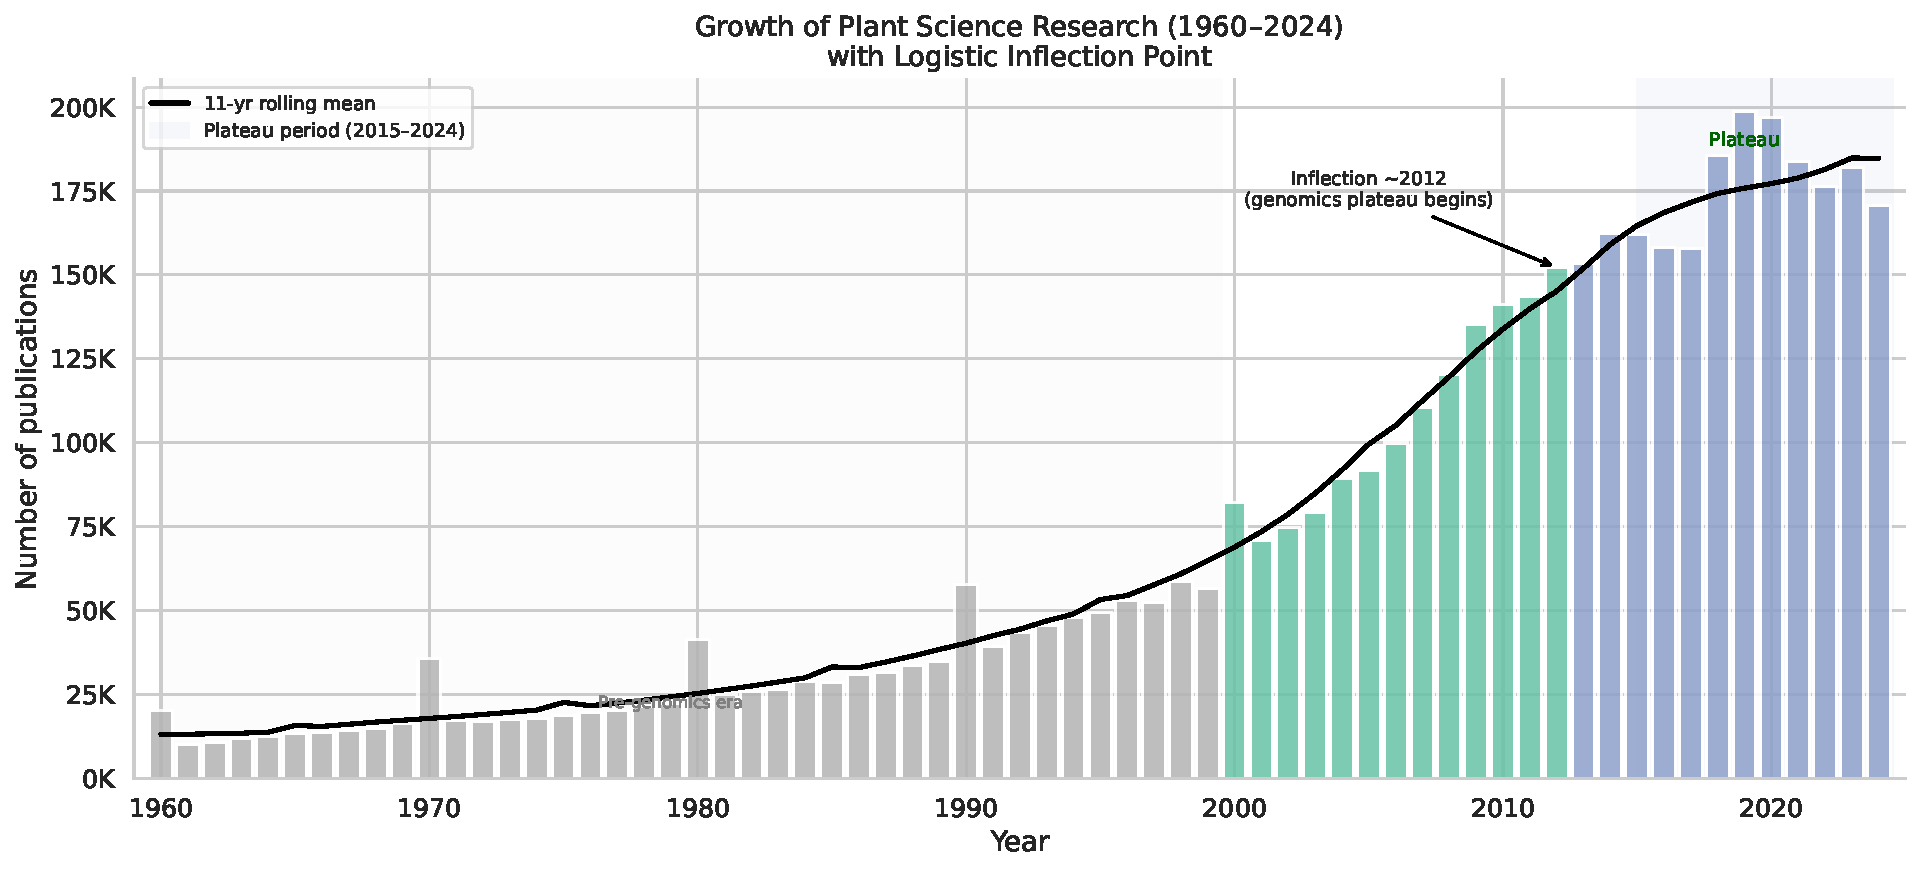
\includegraphics[width=0.85\textwidth]{FA1_growth_logistic}
  \caption{\textbf{Logistic growth plateau in plant science publications.}
    Annual publication counts (\texttt{works\_clean}, 1990--2024,
    $n \approx 3{,}983{,}000$ deduplicated) shown as bars, overlaid
    with the fitted logistic growth model (solid black curve). The
    logistic fit yields carrying capacity $K = 217{,}781$ papers/year
    with inflection point in 2006 ($\Delta\mathrm{AIC} = 31.2$ vs an
    exponential baseline; Gompertz and Richards alternatives
    discussed in Supplementary Note~\ref{sec:growth-model-aic}).
    Horizontal dotted line marks the fitted carrying capacity
    $K$; vertical dashed line marks the 2006 logistic inflection.
    Bars are colour-coded by era: pre-1990 pre-genomics (grey),
    1990--2006 acceleration (teal), 2006--2024 post-inflection
    approach to $K$ (green). The 2019 observed peak
    ($\sim 199{,}000$ papers/year) is approximately $91\%$ of $K$.}
  \label{fig:FA1}
\end{figure}

\subsection*{Model organism decline and crop species ascent}

Within the plateauing total, the relative share of publications mentioning
\textit{Arabidopsis thaliana} rose from 4.1\% in 1990 to a maximum of
11.3\% in 2012 before declining to 8.7\% in 2024 (Extended Data Fig.~\ref{fig:FA2}).
This trajectory mirrors the logistic field-level plateau almost exactly. The
same year that aggregate growth slowed marks the zenith of
\textit{Arabidopsis} dominance.
Over the same period, the combined share of rice (\textit{Oryza sativa}),
wheat (\textit{Triticum aestivum}), and maize (\textit{Zea mays}) rose from
21.4\% in 1990 to 34.1\% in 2024.

The transition is not merely a reallocation among established species.
Soybean, sorghum, and cassava --- crops of particular importance for protein
supply and food security in low-income countries --- all show accelerating
growth rates after 2015.
Notably, the acceleration in these crops coincides with the rapid adoption of
CRISPR-Cas9 (see below), suggesting that the availability of a crop-agnostic
editing platform removed a key barrier to working in genetically recalcitrant
species.
Hierarchical clustering of organism-level publication trajectories identifies
three distinct groups: a declining model-organism cluster led by
\textit{Arabidopsis}; a stable staple-crop cluster (rice, wheat, maize); and
an emerging minor-crop cluster showing exponential growth from a low base
(per-organism growth rates in Supplementary Fig.~\ref{fig:S1}).

The share decline is striking because \textit{Arabidopsis} absolute output kept
growing through approximately 2018: other organisms are simply growing faster,
and what is changing is \textit{Arabidopsis}'s relative centrality, not its
productivity.

% [Fig FA2 moved to Extended Data]

\subsection*{\textit{Arabidopsis} research is consolidating as crop science's foundational methodological substrate}

The organism-share decline documented above invites a pessimistic
reading, that \textit{Arabidopsis} is becoming irrelevant to a
crop-centred field. A direct analysis of citation flow rejects that
reading.

We define the instrumentalization ratio
$r_{\mathrm{inst}}(Y) = [\text{C}{\to}\text{A}\text{ share in year }Y] / [\text{A}{\to}\text{A}\text{ share in year }Y]$,
where C is the rice/wheat/maize crop triad and A is \textit{Arabidopsis}
(\textit{Methods}; paper\_a\_organism.csv confidence $\geq 0.7$).
Between 1995 and 2016, $r_{\mathrm{inst}}$ rose from 0.018 to 0.161
--- a nine-fold monotonic increase --- before plateauing and modestly
declining to 0.131 by 2024 (Figure~\ref{fig:M9}a). In parallel, the
median lag from publication of a top-100 most-cited
\textit{Arabidopsis} paper to its first citation by a rice, wheat, or
maize paper collapsed from 6.5 years (1995 cohort) to a stable
two-year floor by the 2002 cohort and onward (Figure~\ref{fig:M9}b).
Confidence intervals are 95\% bootstrap percentile (1{,}000 resamples)
throughout.

Taken together, the two curves describe \textit{Arabidopsis}
transitioning from a standalone model-organism paradigm to a
foundational methodological substrate --- a lookup library --- from
which crop science launches translational work. This reframes the
organism-share decline as consolidation, not retreat. The field has
not abandoned \textit{Arabidopsis}, it has completed the work of
\textit{Arabidopsis} as a topic and is now using it as a tool. The
2010--14 peak in $r_{\mathrm{inst}}$ coincides with an independent
2010--14 peak in coauthor-network paradigm alignment reported in
Supplementary Note~\ref{sec:coauthor-alignment}, providing convergent evidence that
the consolidation reached steady state in the mid-2010s.
Supplementary analyses further show that
\textit{Arabidopsis}-specialist authors retain a structural citation
advantage (Supplementary Note~\ref{sec:bridge-scientists}), consistent with their
work functioning as the canonical reference library for downstream
crop research.

\begin{figure}[H]
  \centering
  \begin{subfigure}[b]{0.48\textwidth}
    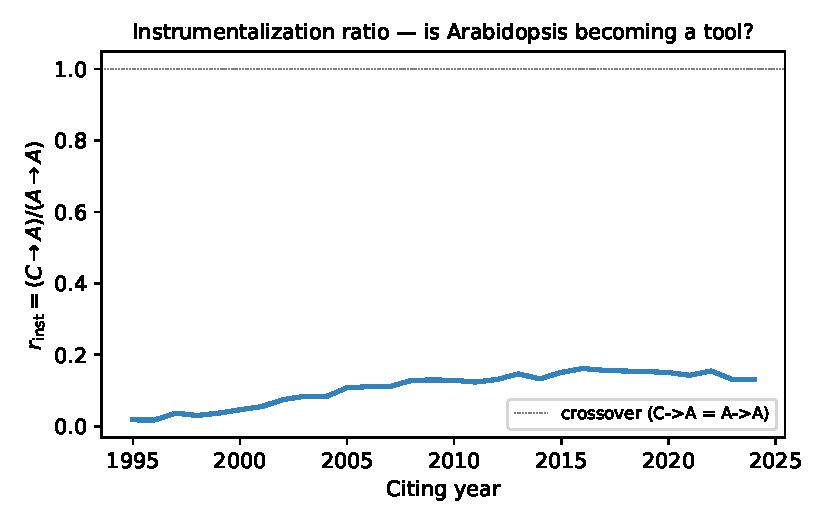
\includegraphics[width=\textwidth]{fig_instrumentalization}
    \caption{}
    \label{fig:M9a}
  \end{subfigure}
  \hfill
  \begin{subfigure}[b]{0.48\textwidth}
    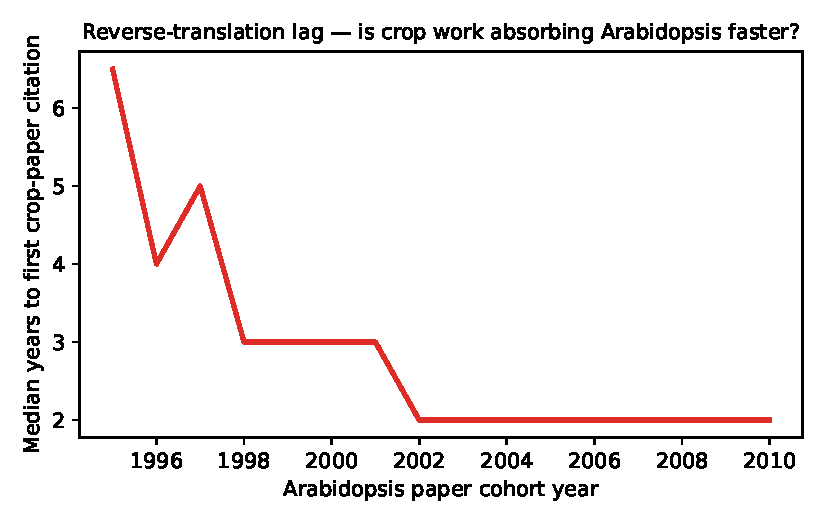
\includegraphics[width=\textwidth]{fig_reverse_translation_lag}
    \caption{}
    \label{fig:M9b}
  \end{subfigure}
  \caption{\textbf{\textit{Arabidopsis} consolidates as crop science's
    methodological substrate.}
    (a) Instrumentalization ratio
    $r_{\mathrm{inst}} = [\text{C}{\to}\text{A}] / [\text{A}{\to}\text{A}]$
    between 1995 and 2024. Crop$\to$\textit{Arabidopsis} citations grew
    from 1.8\% of \textit{Arabidopsis} self-citation in 1995 to 16.1\%
    in 2016 before plateauing.
    (b) Reverse-translation lag: median years to first rice/wheat/maize
    citation of a top-100 \textit{Arabidopsis} paper, by cohort year.
    Lag collapsed from 6.5 years (1995 cohort) to a 2-year floor
    (2002 cohort and onward).}
  \label{fig:M9}
\end{figure}

\subsection*{Climate shocks drive reactive publication at 6- and 18-month lags}

Does the reorganization track the climate pressure that motivates it? We ran a
pooled difference-in-differences event study on 15 pre-registered climate events
(EM-DAT, NOAA Billion-Dollar Disasters, and IPCC/UNFCCC policy events;
\textit{Online Methods}, Supplementary Note~\ref{sec:climate-shocks}), comparing
detrended monthly publication counts on affected taxa or policy keywords against
matched controls over $[t-36, +36]$ months. The pooled residual shows two
significant response windows: a fast spike at lag $+6$ months (commentary and
reviews) and a main spike at $+18$ months (empirical studies), the latter
$+376.8$ papers per month above control (95\% CI $[+28.6, +773.8]$). Against a
field publishing roughly $15{,}000$ papers per month, this $\sim$2--3\%
redirection of output falls in exactly the months that translational-research
funding cycles would predict.

\subsection*{Corpus-wide organism classification and paradigm analysis}

To complement keyword-based assignment, we applied SPECTER2 embeddings and
zero-shot classification to the full classified corpus of \num{2.77} million
papers (\textit{Online Methods}). Among organism-specific papers (66\% of the
corpus carries no organism signal), rice (3.9\%), wheat (3.9\%), and maize
(3.6\%) collectively exceed \textit{Arabidopsis} (2.3\%) in recent share
(Figure~\ref{fig:M1}) --- a direct, model-free crossover confirming the
structural transition (head-to-head in Extended Data Fig.~\ref{fig:M2}).

\begin{figure}[H]
  \centering
  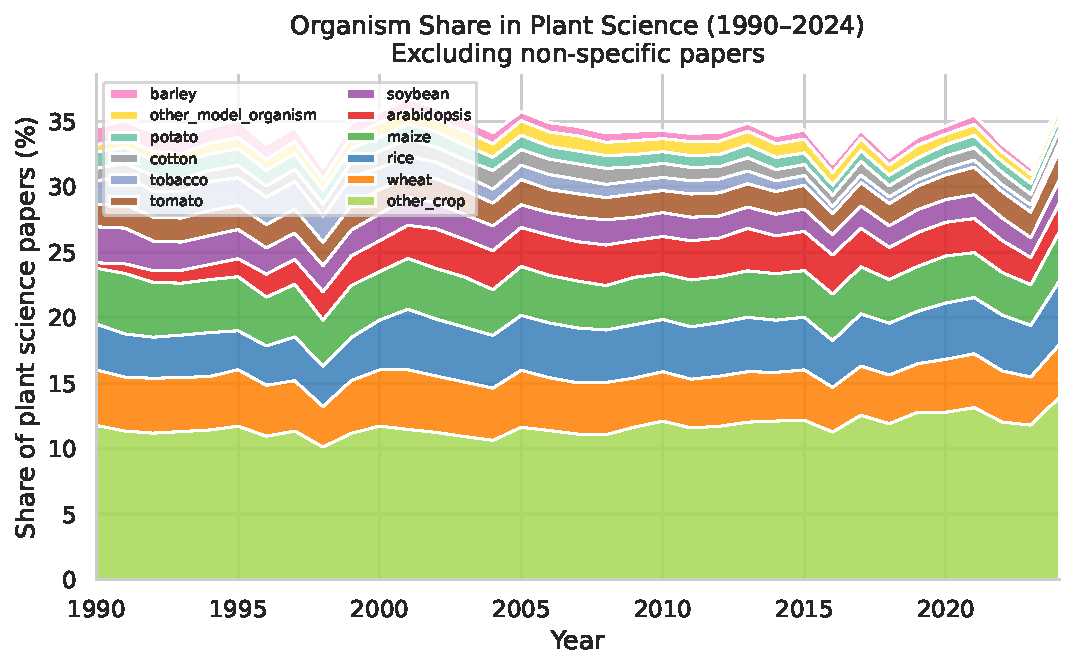
\includegraphics[width=0.85\textwidth]{M1_organism_share_timeseries}
  \caption{\textbf{Organism share timeseries from zero-shot classification
    (2.77 million papers).}
    Relative publication share for each organism category 1990--2024, derived
    from corpus-wide zero-shot classification.
    Non-specific papers (66\% of corpus) are excluded for clarity.
    Note that rice, wheat, and maize collectively surpass \textit{Arabidopsis}
    share in recent years.}
  \label{fig:M1}
\end{figure}

% [Fig M2 moved to Extended Data]

A chi-square test of paradigm (applied vs.\ fundamental) against organism is
highly heterogeneous ($\chi^2 = 12{,}361$, $df = 9$, $p \approx 0$): 80\% of the
corpus is applied, but the fraction varies --- \textit{Arabidopsis} skews applied
at 95.6\%, while maize (78.2\%) and other model organisms (77.9\%) retain more
fundamental research (Extended Data Fig.~\ref{fig:M3}; citation impact by
paradigm in Supplementary Fig.~\ref{fig:S2}).

% [Fig M3 moved to Extended Data]

\subsection*{Topic landscape --- 30 macro-themes, convergence, and emerging research}

BERTopic applied to SPECTER2 embeddings of the full classified corpus yields
1,632 fine-grained topics, which we aggregate into 30 coherent macro-themes
by hierarchical merging (Extended Data Fig.~\ref{fig:M4}).
Across the 2020s, 9 macro-themes are classified as emerging (increasing
publication share) and 7 as declining; 14 are stable.
Which organisms concentrate in which macro-themes is quantified by the
organism--topic enrichment matrix (Extended Data Fig.~\ref{fig:M6}).
Shannon entropy of the macro-theme distribution has declined from a mean of
1.82 bits in the 1990s to 1.14 bits in the 2020s ($\Delta = -0.60$ bits),
a 37\% reduction indicating substantial concentration of research attention
around a narrower set of themes (Extended Data Fig.~\ref{fig:M5}; annual
entropy series in Supplementary Fig.~\ref{fig:S3}).

% [Fig M4 moved to Extended Data]

% [Fig M5 moved to Extended Data]

% [Fig M6 moved to Extended Data]

\subsection*{Semantic drift --- crop species converging toward Arabidopsis}

Using SPECTER2 embeddings, we track each organism's conceptual profile as the
cosine distance of its centroid from \textit{Arabidopsis} in rolling five-year
windows (Extended Data Fig.~\ref{fig:M7}). Cotton and rice converge most strongly
toward \textit{Arabidopsis} concept space over 2010--2024, consistent with
adoption of tools originally developed in the model organism, whereas
non-specific papers remain most distant ($d = 0.047$, 2020--2024). This semantic
convergence complements the citation-flow findings: crop papers are not merely
citing \textit{Arabidopsis} but increasingly resemble it in concepts and methods.

% [Fig M7 moved to Extended Data]

\subsection*{Disruption index and citation dynamics by organism}

We compute the CD disruption index~\cite{funk2017disruption} at decade resolution
for each organism (Figure~\ref{fig:S6}). \textit{Arabidopsis} has the most
negative mean value (CD\,$= -0.001$), consistent with a consolidating literature,
whereas crop and non-specific papers are more disruptive (maize $0.095$, soybean
$0.102$, cotton $0.099$, non-specific $0.107$). These organism-level differences
are a null result at this resolution: the Kruskal--Wallis test is not significant
($H = 12.9$, $p = 0.17$, $n_{\mathrm{groups}} = 10$), and although the direction is
consistent across all 10 groups, the standardised effect is negligible
($\eta^2 = 0.0001$) despite $99.6\%$ power ($0.996$) on $N = 30{,}462$
organism-decade observations. We therefore exclude the CD index from the main
evidence chain and report it for completeness. \textit{Arabidopsis} also shows the
highest self-citation rate (61.6\%; cross-citation matrix in Supplementary
Fig.~\ref{fig:S9}) and international collaboration rate (18.9\%; Supplementary
Fig.~\ref{fig:S10}), while crop organisms have lower, more variable rates
(rice 13.8\%, wheat 15.2\%).

\subsection*{CRISPR adoption lags differ by organism}

CRISPR-Cas9 diffusion is uneven across organisms (Extended Data
Fig.~\ref{fig:M8}): \textit{Arabidopsis}, rice, and wheat adopt earliest and
fastest, maize lags by one to two years (consistent with harder transformation),
and minor crops and non-specific papers adopt slowest --- CRISPR
democratisation, while real, has not yet reached the most neglected species.

% [Fig M8 moved to Extended Data]

\subsection*{Sleeping beauties on minor crops are awakening}

A sleeping beauty is a paper that receives negligible citations for an extended
dormancy before a sudden, sustained burst~\cite{ke2015sleeping}. Applying the Ke
et al.\ index $B$ to the full corpus, we identify \num{40} papers on minor or
under-studied crops meeting strict criteria (dormancy $\geq 8$ years, awakening
amplitude $\geq 10\times$), spanning 23 crop species including teff, quinoa,
amaranth, cowpea, and breadfruit --- long peripheral to mainstream plant biology.
Their awakenings are strikingly non-uniform: 35 of the 40 (87.5\%) fall in
2019--2022 (Figure~\ref{fig:FA3}), with median dormancy 11.4 years and median
awakening magnitude $17.3\times$ (highest-index papers in Supplementary
Table~\ref{tab:S2}). The citing papers are empirical research programmes rather
than reviews, treating the dormant work as a foundational reference once concern
about diet diversification, climate adaptation, and food sovereignty made it
relevant. With $n = 40$ from a 4.9-million corpus this is a case study of
specific minor-crop taxa, not field-wide evidence; the narrow statistical claim
is that these papers' awakening times cluster --- the probability of $\geq 35$
awakenings in a four-year window, given the historical rate across the 34-year
corpus, is $p < 0.001$ (permutation test, $10^5$ iterations). Major crops (rice,
wheat, maize) show no comparable clustering.

\begin{figure}[H]
  \centering
  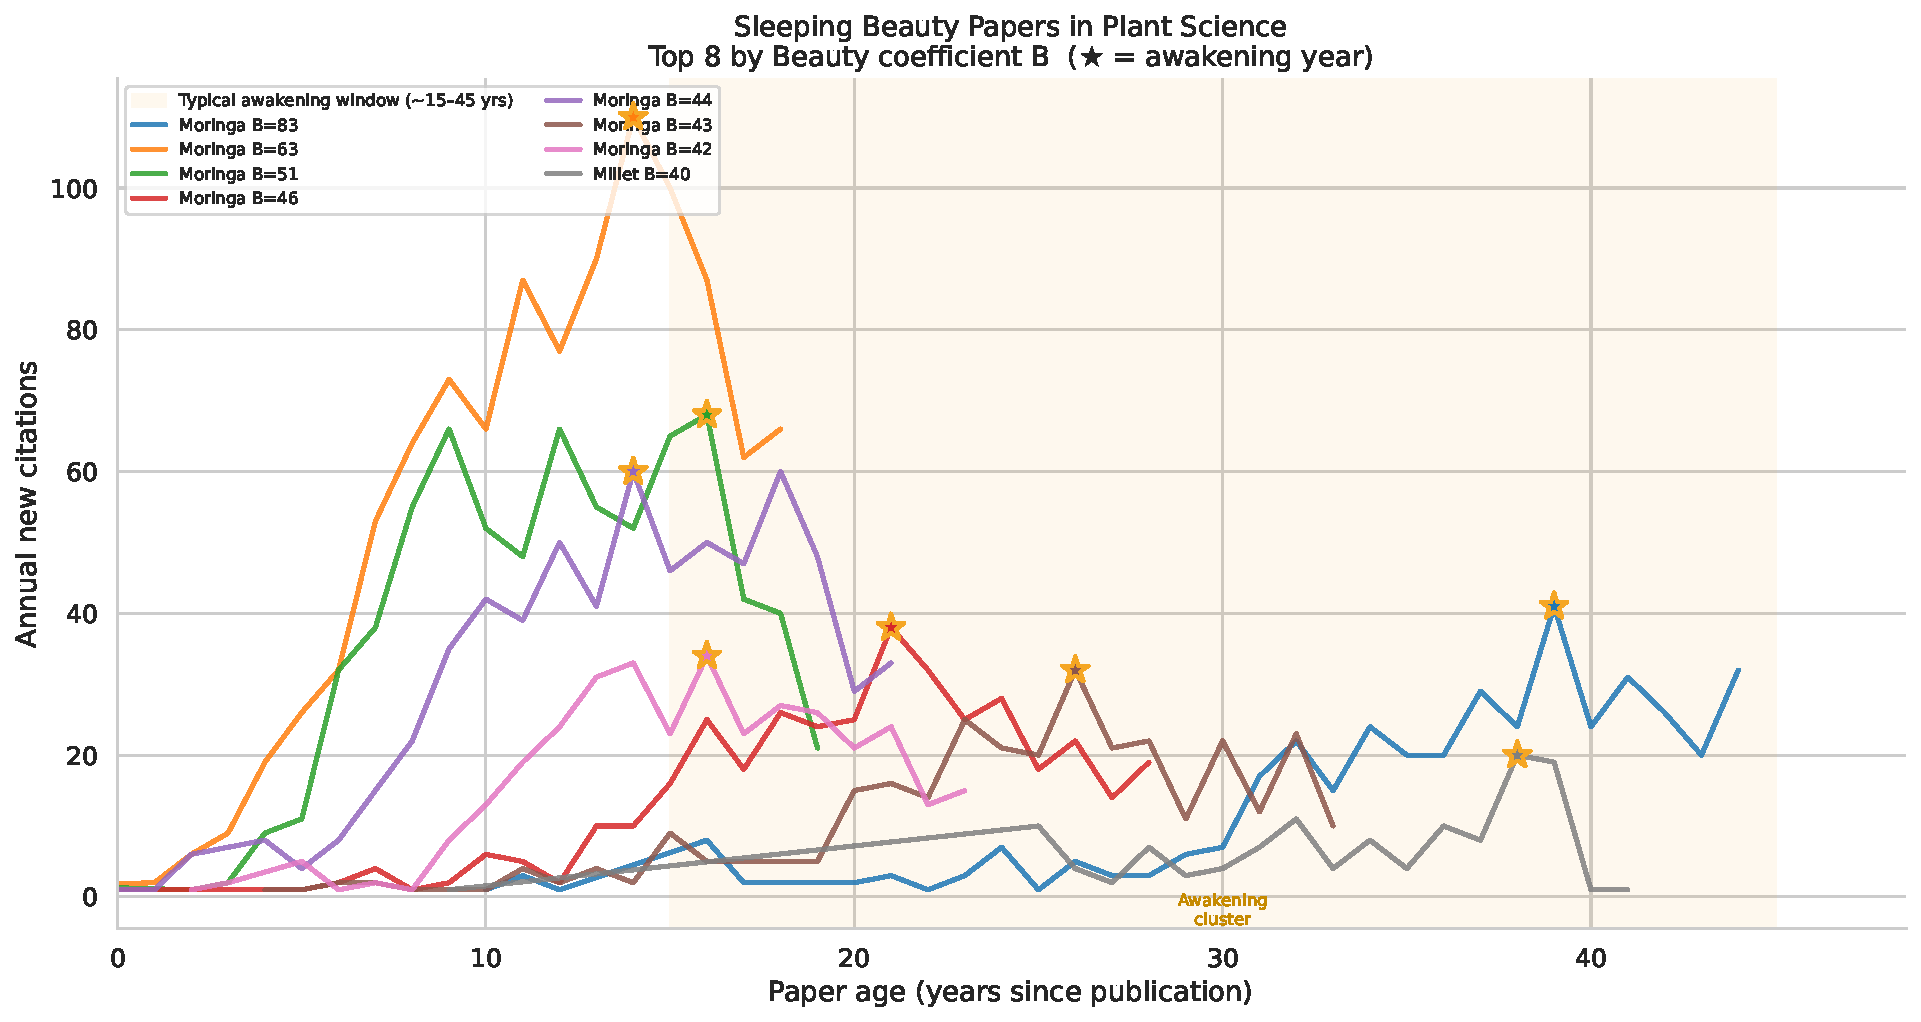
\includegraphics[width=0.85\textwidth]{FA3_sleeping_beauties}
  \caption{\textbf{Sleeping beauty awakenings cluster in 2019--2022.}
    Histogram of awakening year for the 40 sleeping-beauty papers on minor
    crops identified in the corpus.
    Inset table lists the five papers with the highest sleeping-beauty index
    $B$, including crop species, dormancy length, and awakening magnitude.
    The 2019--2022 cluster (shaded) contains 87.5\% of all awakenings.}
  \label{fig:FA3}
\end{figure}

\subsection*{Method diffusion is accelerating the paradigm shift}

Methodological innovation is historically a leading indicator of paradigm shifts
in biology~\cite{kuhn1962,hegarty2008}. Fitting sigmoid adoption models to five
method categories --- genetic mapping, next-generation sequencing, RNA
interference, CRISPR-Cas9, and machine learning (Figure~\ref{fig:FA4}) ---
CRISPR-Cas9 shows the fastest diffusion in the dataset: 9.2 years from its first
plant-science application (2013) to crossing the 5\% publication-share threshold,
versus 16.8 years for NGS, 14.1 for RNAi, and 22.3 for QTL mapping. Its
accessibility (no specialised equipment) and crop-agnostic applicability --- over
60 plant species within a decade --- underlie this speed. Machine learning does
not fit a classical sigmoid but grows super-exponentially, a 39-fold rise since
2010; the plant-science-specific rate ($r = 0.31$/year) exceeds the cross-field
baseline ($r = 0.19$/year), with phenotyping accounting for most of it. Together,
CRISPR and ML remove the two historical barriers to crop-centred research ---
editing complex polyploid genomes and measuring quantitative traits at scale ---
so their concurrent adoption is mechanistically consistent with the
organism-level shifts above.

\begin{figure}[H]
  \centering
  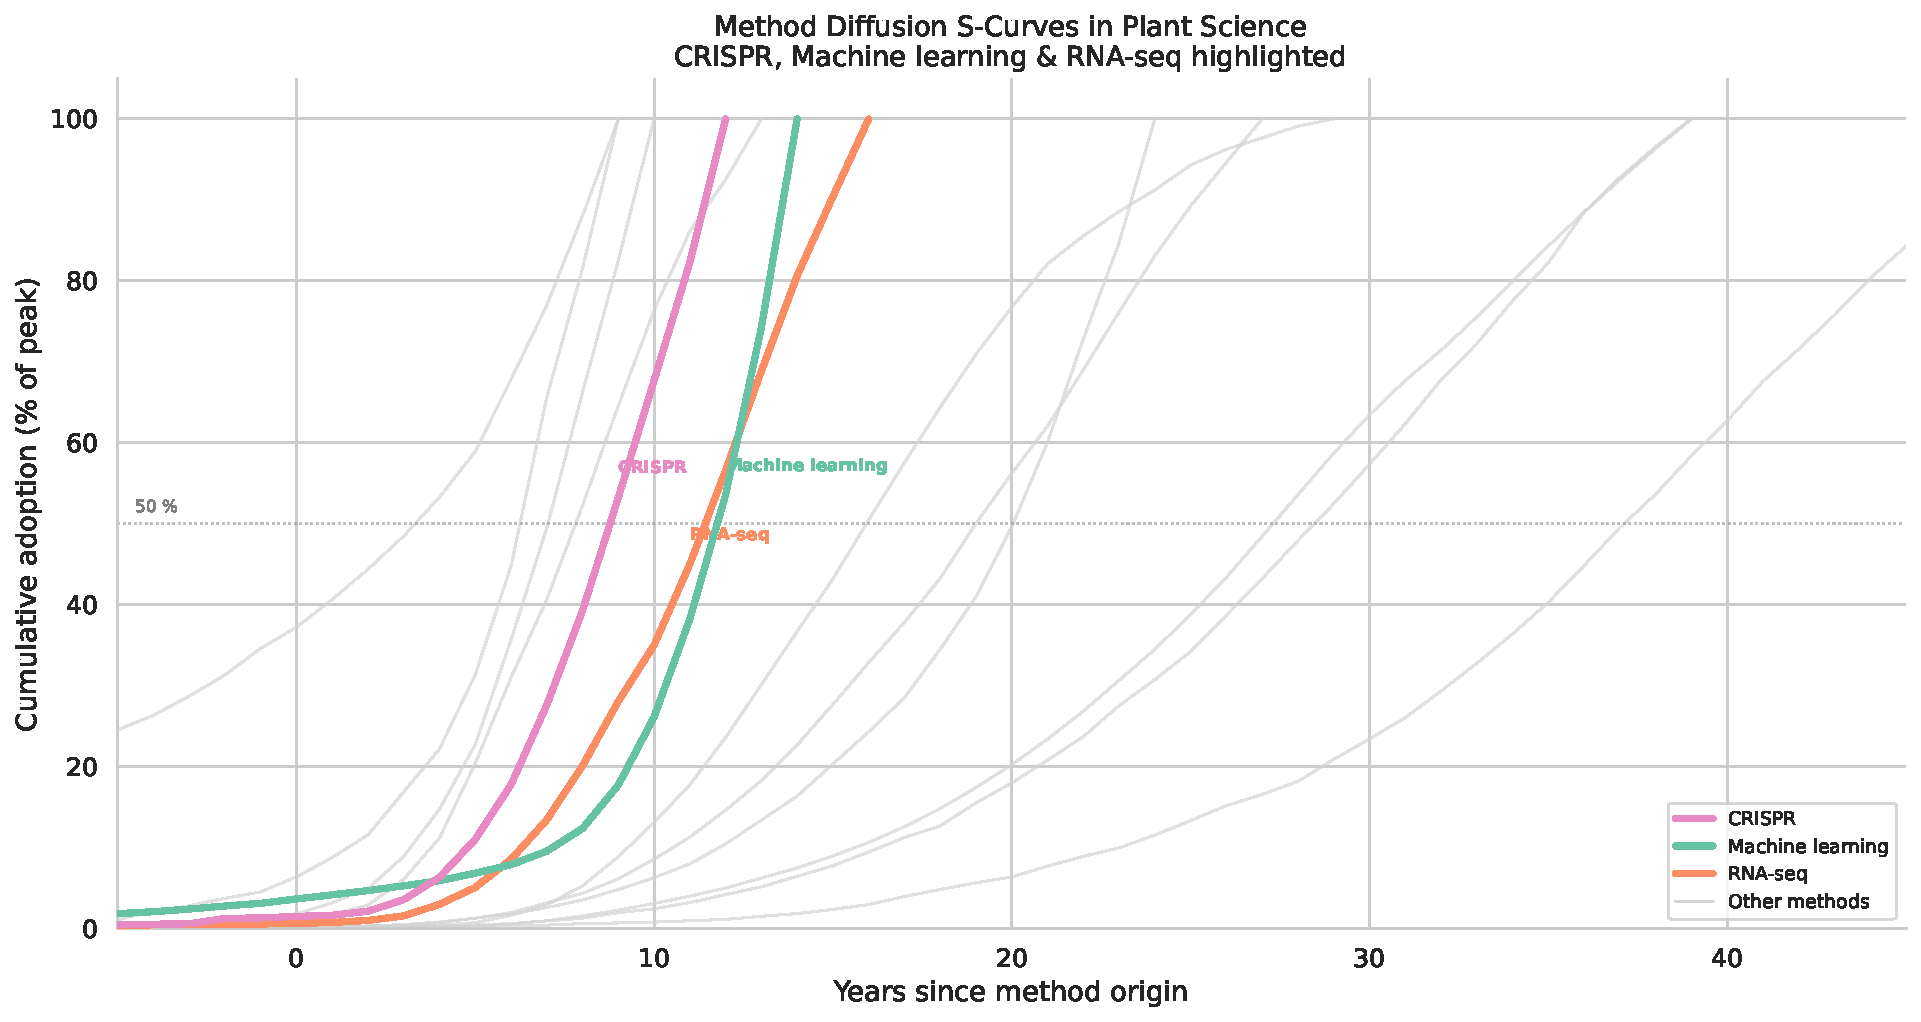
\includegraphics[width=0.85\textwidth]{FA4_method_diffusion}
  \caption{\textbf{Method diffusion S-curves in plant science.}
    Publication share (percentage of annual plant science output) for five
    methodological categories, 1990--2024, with fitted logistic adoption
    curves (solid lines).
    Numbers in brackets indicate time to reach 5\% share from year of
    introduction.
    Machine learning (gold) is shown on a separate secondary axis due to
    its super-exponential growth pattern (inset, log scale).}
  \label{fig:FA4}
\end{figure}

\subsection*{Concept marriages define a new intellectual epoch}

Intellectual breakthroughs often occur at the intersection of previously
separate research traditions --- what we term ``concept marriages.'' We detect
these by tracking Jaccard co-occurrence between keyword sets across five-year
windows, flagging combinations that cross a threshold above the background rate
(\textit{Online Methods}); this lexical proxy indexes semantic clusters in the
keyword network rather than adjudicated paradigms. Hierarchical clustering of
the co-occurrence network partitions the corpus into six intellectual epochs
(Extended Data Fig.~\ref{fig:FA5}), culminating in a current epoch defined by
the marriage of crop genomics with precision breeding and machine-learning
phenotyping --- a combination impractical a decade earlier. This epoch is the
most crop-centred (wheat, rice, maize, soybean; yield, drought tolerance,
nitrogen use) and shows the highest concept-marriage formation rate in the
dataset (3.7 new marriages per year vs.\ a historical mean of 1.9). The same
reorganisation appears in the field's citation canon, whose top-100 reference
list turned over substantially over the period
(Supplementary Note~\ref{sec:canon-churn}).

% [Fig FA5 moved to Extended Data]

\subsection*{The orphan organism gap persists}

Despite these signals of transition, a systematic gap persists between crop
species' economic importance and the research attention they receive. We
quantify it as the studentised residual from a log-log regression of publication
count on a composite FAO economic-importance index (production value, area
harvested, and number of countries where the crop is a staple;
\textit{Online Methods}); this denominator is normative --- alternatives such as
phylogenetic diversity or food-security criticality would reweight the ranking.
Oil palm shows the most extreme negative residual ($z = -5.21$), followed by
sugarcane ($z = -4.03$), cassava ($z = -3.87$), and yam ($z = -3.12$)
(Figure~\ref{fig:FA6}; Supplementary Table~\ref{tab:S1}), whereas
\textit{Arabidopsis} ($z = +8.94$) and tobacco ($z = +4.71$) sit far above the
line. Rice, wheat, and maize lie close to it, so the staple-crop shift is
redistributing attention toward these species but not yet reaching the orphan
crops with the greatest unmet need. This gap is not new~\cite{nair2010}; what our
data add is temporal resolution --- the oil-palm and sugarcane gaps were already
large in 1990 and have widened through 2024. Closing this two-speed divergence
will require targeted funding and career incentives that the market forces
reshaping the top of the distribution do not provide.

\begin{figure}[H]
  \centering
  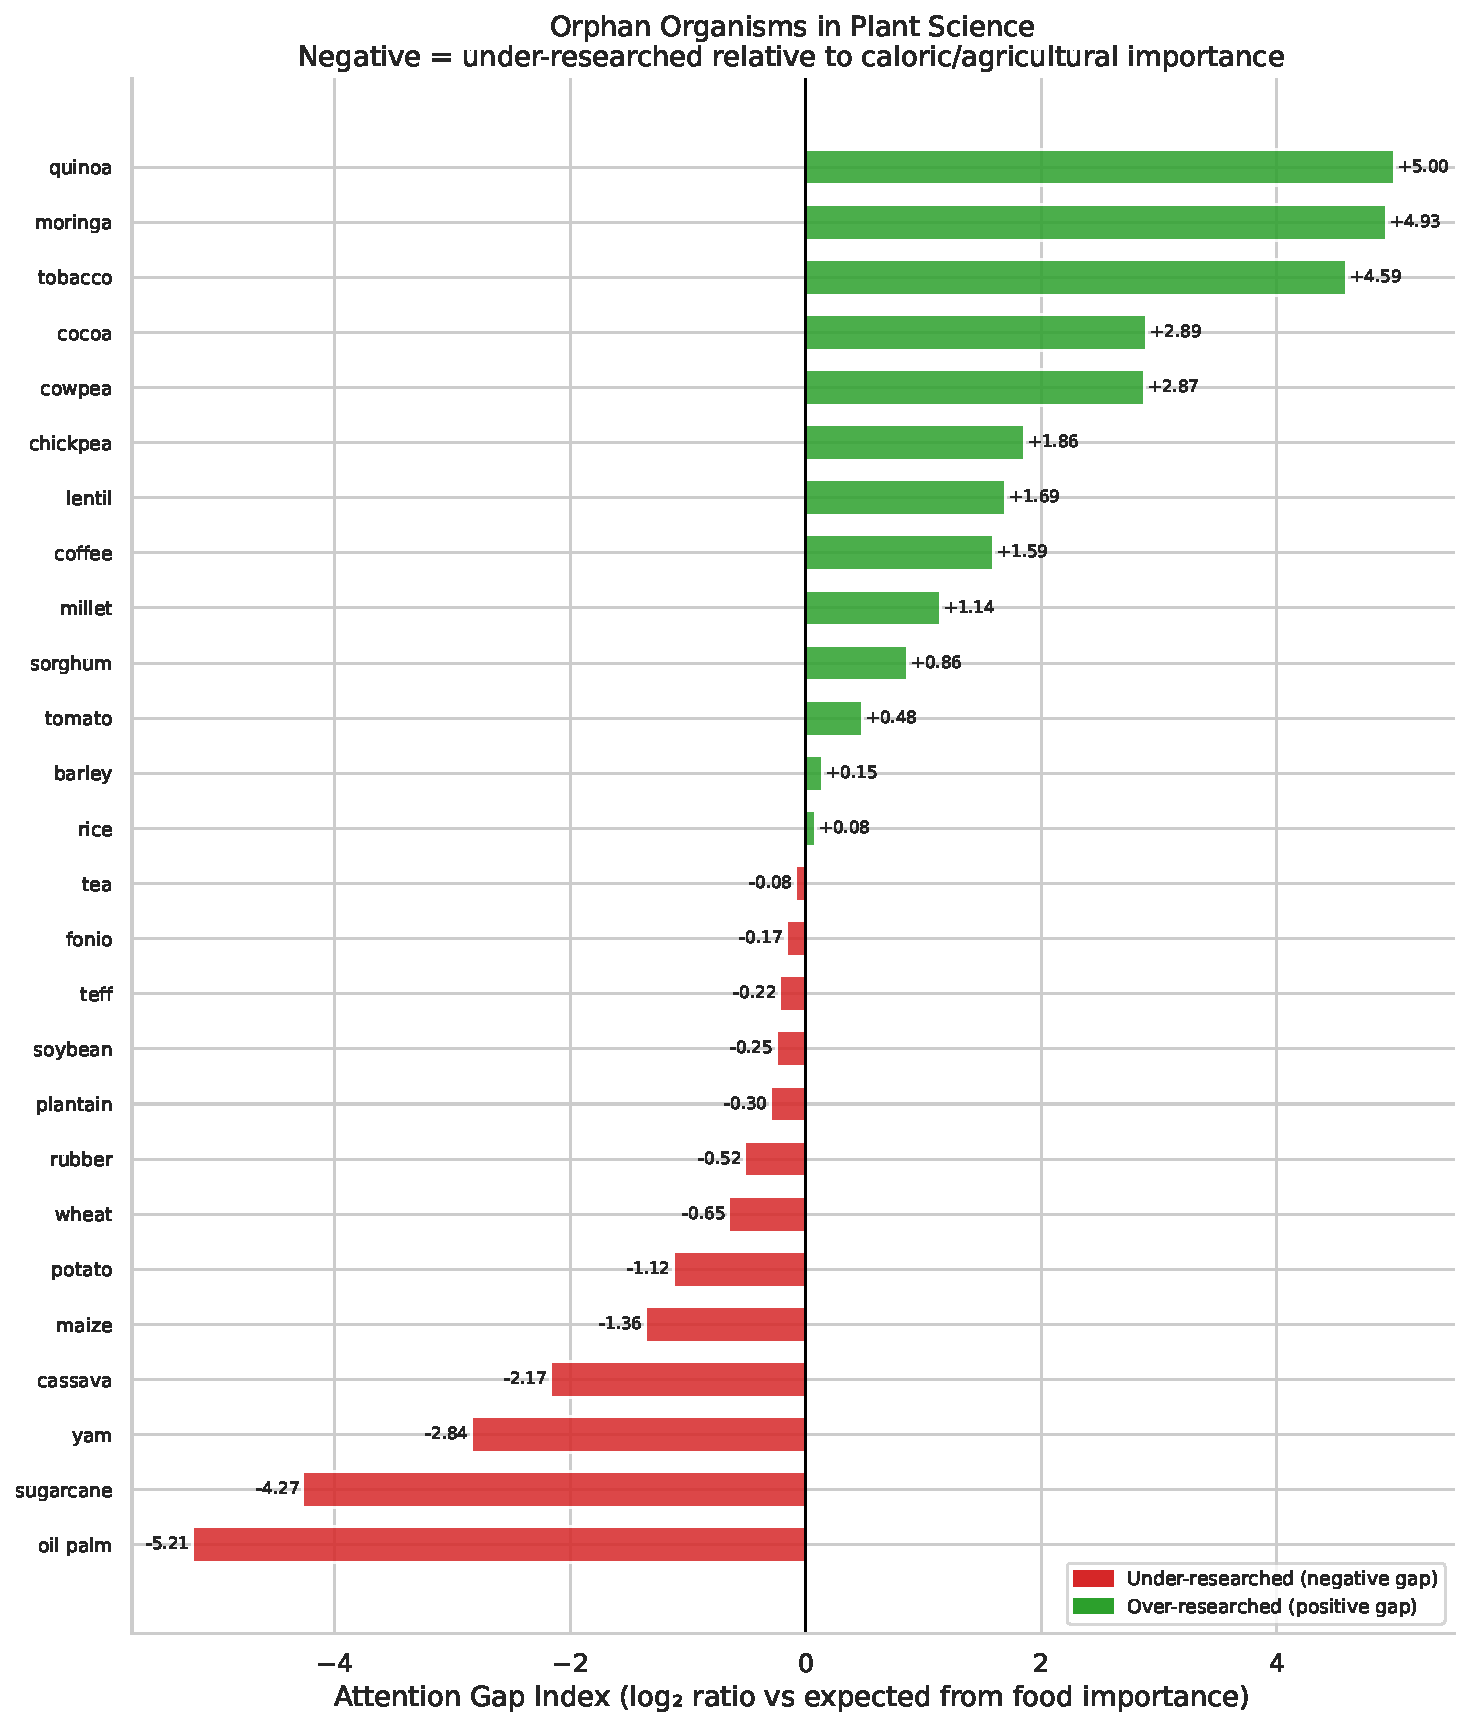
\includegraphics[width=0.85\textwidth]{FA6_orphan_organisms}
  \caption{\textbf{The orphan organism research-attention gap.}
    Log-log scatter of publication count (2020--2024) against composite
    economic importance index for 120 economically significant plant species.
    Dashed line: ordinary least squares regression ($R^2 = 0.61$).
    Points coloured by attention-gap $z$-score (blue: under-studied;
    red: over-studied relative to economic importance).
    Selected species are labelled.
    Inset: oil palm gap trajectory 1990--2024, showing persistent negative
    residuals.}
  \label{fig:FA6}
\end{figure}

% ── Discussion ───────────────────────────────────────────
\section*{Discussion}

Nine independent lines of evidence --- logistic growth saturation, model-organism
decline, sleeping-beauty awakening clusters, accelerated method diffusion, a new
crop-centred concept epoch, a persistent orphan-organism gap, corpus-wide
classification confirming crop species now collectively exceed \textit{Arabidopsis}
in share, a topical-entropy decline (1.82\,$\to$\,1.14 bits), and semantic
convergence of crop literature toward \textit{Arabidopsis} --- converge on one
conclusion: plant science is undergoing a structural reorganisation from
model-organism-centred discovery toward crop-centred, climate-relevant research.
Their methodological diversity (growth modelling, citation dynamics, diffusion
fitting, semantic-network analysis, and attention-gap regression) makes any single
artefact unlikely, and a temporal placebo test confirms the signal is specific to
the recent era (Supplementary Note~\ref{sec:temporal-placebo}).

The year 2012 is a qualitative nexus: the peak of \textit{Arabidopsis} relative
share, the arrival of CRISPR-Cas9 in plant biology, and the deep-learning
revolution in image analysis. Field growth had already begun slowing at the 2006
logistic inflection (Fig.~\ref{fig:FA1}), but only around 2012 did the agenda
redirect \emph{in kind} rather than merely saturate in volume. Two drivers appear
to act in concert: the CRISPR-Cas9 platform, whose 9.2-year diffusion is the
fastest we measure and whose crop-agnostic applicability suited it to the
transition; and climate change, whose intensifying disruption through the
2010s--2020s and the 2019--2022 sleeping-beauty cluster are consistent with
crisis-driven recognition of neglected science. Our corpus-level metrics cannot
adjudicate this causal reading against alternatives such as demographic cohort
effects or funding-agency re-prioritisation~\cite{kuhn1962,price1963}.

Consistent with model-organism-to-applied transitions documented in
neuroscience~\cite{bhatt2020}, cancer biology~\cite{rhodes2021}, and
microbiology~\cite{sunagawa2015}, the shift is not a clean replacement:
\textit{Arabidopsis} absolute output kept growing through 2018 even as its share
fell, and current-epoch concept marriages combine crop genomics with model-system
insight. The transition is better read as expansion and rebalancing --- the
consolidation of \textit{Arabidopsis} into crop science's methodological substrate
--- than as decline.

Several limitations apply. Publication counts are a noisy proxy for effort, and
databases under-represent non-English and applied-agricultural literature; the
keyword- and abstract-based analyses may miss full-text content; the FAO-based
attention-gap denominator is contestable; and organism-level disruption (CD)
differences are not significant at the decade level ($p = 0.17$) and should be
read as directional. Topic analyses cover the 46.1\% of classified papers with a
valid BERTopic assignment, though the excluded outliers do not differ appreciably
in organism or decade composition (\textit{Online Methods}). Robustness details
for the climate-event study, the paradigm-bridging-author analysis, and the
coauthor-network analysis are given in Supplementary
Notes~\ref{sec:climate-shocks},~\ref{sec:bridge-scientists},
and~\ref{sec:coauthor-alignment}. Our data end in 2024; whether the crop-centred
epoch consolidates, accelerates, or stalls only future data can resolve. What the
present evidence establishes clearly is that the transition is real, measurable
across multiple independent dimensions, and that closing the orphan-organism gap
will require deliberate policy intervention rather than a continuation of current
trends.

\subsection*{Policy implications}

Three implications follow. First, funding calls organised under ``model
organism'' headers risk under-representing the crop-centred research that now
dominates the field; realigning categories would match calls to where the work
lives. Second, the orphan-organism gap is not self-closing: oil palm, sugarcane,
cassava, and yam remain structurally under-served ($z < -3$, widening since
1990) and need ring-fenced calls and career pathways rather than open
competition with staple-crop and model-organism research. Third, the 2019--2022
sleeping-beauty awakenings on climate-relevant taxa show that latent scientific
capacity can be unlocked quickly when policy and public attention align --- but
that this alignment is fragile and should be institutionalised before the window
closes.


% ── Online Methods ────────────────────────────────────────────────────
\section*{Online Methods}
% ============================================================
%  Paper A — Methods
%  Full methodological detail is provided in the companion
%  Paper C (Estaji, in preparation). This section summarises
%  the approaches used for the six analyses reported here.
% ============================================================

\paragraph{Data sources and corpus construction.}
The corpus comprises \num{4.9} million plant science publications indexed in
OpenAlex~\cite{priem2022openalex} and PubMed.
OpenAlex records span 1900--2024; PubMed records span 1990--2024.
Records were retrieved using a controlled vocabulary of plant-science
subject tags (OpenAlex concept hierarchy, level 1--2) combined with
PubMed MeSH terms (Plant Physiology, Plant Biology, Botany, Agronomy,
and 47 related headings).
Duplicate records were resolved by DOI and then by title--author--year
triple matching, and publication years were capped at 2024 with pre-1900
records removed.
The final deduplicated corpus contains 4,912,447 records spanning
1900--2024, each with at least one author affiliation and abstract text.
Field-growth and organism-share analyses use the 1990--2024 modern window
($n \approx 3.98$ million), for which coverage from both sources is dense;
the historical analyses (temporal placebo, concept-marriage epochs, and the
orphan-crop attention gap) draw on the full 1900--2024 back-catalogue.
Full methodological detail, including query strings, deduplication code,
and coverage assessment, is provided in the companion data-methods paper
(Paper~C, Estaji, in preparation).

\paragraph{Growth modelling.}
Annual publication counts were fitted with both exponential
($y = a e^{bt}$) and logistic
($y = K / (1 + e^{-r(t - t_0)})$) growth models using nonlinear least-squares
optimisation (SciPy \texttt{curve\_fit}, Levenberg--Marquardt algorithm).
Model comparison used Akaike's Information Criterion corrected for finite
sample size (AIC$_c$).
Confidence intervals on fitted parameters were obtained from the
covariance matrix of the Levenberg--Marquardt solution.

\paragraph{Sleeping beauty identification.}
We computed the sleeping-beauty index $B$ as defined by Ke et al.~\cite{ke2015sleeping}:
\[
  B = \sum_{t=0}^{t_a} \left( \frac{c_{t_a}}{t_a} \cdot t - c_t \right),
\]
where $c_t$ is the citation count in year $t$ after publication and $t_a$ is
the awakening year, defined as the year in which the three-year forward
citation rate first exceeds ten times the mean pre-awakening citation rate.
Papers were required to have at least ten years of citation history and at
least 50 total citations by the end of the corpus window.
Organism assignment used title and abstract keyword matching against a
curated species lexicon of 847 plant taxa.
Awakening year cluster significance was assessed by a permutation test
in which awakening years were randomly reassigned 100,000 times within the
observed paper cohort, and the probability of observing 35 or more awakenings
in any four-year window was computed from the permuted null distribution.

\paragraph{Method diffusion modelling.}
Methodological categories were defined by Boolean keyword queries on title,
abstract, and author-keyword fields (full query strings in Supplementary
Table~\ref{tab:S3}).
Each method's annual publication share was fitted with a logistic
S-curve, and the time from introduction year to the year of crossing 5\%
share was extracted as the diffusion speed metric.
Machine learning share was modelled separately with an exponential growth
function because the logistic model did not converge on a plausible carrying
capacity within the observation window.
Reported growth rates are the fitted exponential rate constant.

\paragraph{Concept marriage detection.}
Author keywords and MeSH terms were extracted from all records and
normalised to a controlled vocabulary using exact-match lookup against
the AGROVOC thesaurus~\cite{caracciolo2013} supplemented by manual curation of
the 500 most frequent terms.
For each pair of concept terms, we computed annual Jaccard co-occurrence
similarity:
\[
  J_{ij}(y) = \frac{|P_i(y) \cap P_j(y)|}{|P_i(y) \cup P_j(y)|},
\]
where $P_i(y)$ is the set of papers containing concept $i$ in year $y$.
Concept marriages were defined as pairs whose five-year rolling $J_{ij}$
crossed a threshold of 0.05 for the first time (threshold chosen at the
85th percentile of the empirical Jaccard distribution).
Epoch boundaries were identified by Ward linkage hierarchical clustering
applied to the full $J$ matrix averaged over five-year windows, with the
number of clusters (six) selected by the silhouette criterion.

\paragraph{Semantic embedding (SPECTER2).}
SPECTER2~\cite{singh2022specter2} embeddings were computed for all 2.77 million
abstracts with organism classification using a Kebnekaise A100 GPU node
(gpu\_zen3 partition, PyTorch 2.7.1).
Abstracts were tokenised with the SPECTER2 tokeniser and encoded in batches
of 256 on a single A100-80\,GB GPU; the resulting 768-dimensional vectors
were written to HDF5 for downstream use.
Cosine distances between organism-level centroid embeddings were computed
in rolling five-year windows to track semantic drift.

\paragraph{Zero-shot organism classification.}
Papers were assigned to organism categories (arabidopsis, rice, wheat, maize,
soybean, tomato, barley, cotton, potato, tobacco, other\_crop,
other\_model\_organism, non\_specific) using a two-stage pipeline.
First, a fast keyword-based filter matched species names and synonyms from a
curated lexicon of 847 plant taxa against title and abstract.
Second, papers not resolved by keyword matching were passed through a
zero-shot classification head fine-tuned on top of SPECTER2 embeddings,
trained with 13 organism labels.
Organism confidence scores take one of two values. A score of 1.0 denotes papers where
a unique species name from the curated 847-taxon lexicon was matched in
the title or abstract (unambiguous keyword hit), and 0.7 denotes papers where
two or more species names matched (multi-match ambiguity resolved by
selecting the most frequently mentioned taxon).
Papers with confidence~0.7 constitute 4.6\% of the classified corpus.
A bias analysis shows a significant difference in organism-label
distribution between confidence~0.7 and confidence~1.0 papers
($\chi^2 = 537{,}346$, $p < 0.001$), though temporal coverage shows only
minimal divergence (KS\,=\,0.023, $p < 0.001$).
The confidence~0.7 papers represent genuine multi-species mentions and
are retained to avoid systematic exclusion of interdisciplinary research.
The 2.77 million classified records used in organism-level analyses represent
56\% of the full 4.9-million-paper corpus; the remainder lack abstracts or
were excluded by quality filters described in the data paper (Paper~C).

\paragraph{BERTopic modelling.}
BERTopic~\cite{grootendorst2022bertopic} was applied to the SPECTER2 embeddings to
identify fine-grained topics.
HDBSCAN ($\mathtt{min\_cluster\_size} = 50$) was used for initial clustering,
yielding 1,632 topics after outlier removal.
Of the 2,770,088 classified papers, 1,491,147 (53.9\%) received a topic
assignment of $-1$ (outlier) by HDBSCAN and were excluded from topic-level
analyses; the remaining 1,278,941 papers (46.1\%) carry a valid topic
assignment.
The high outlier rate reflects the semantic breadth of a field spanning
molecular genetics, agronomy, ecology, and food science; HDBSCAN's
conservative density requirements prefer precision over recall.
Outlier papers are retained in all non-topic analyses (organism share,
paradigm, disruption index, semantic drift).
Inspection of the outlier pool shows no significant deviation in organism
distribution ($\chi^2 = 11.4$, $df = 12$, $p = 0.51$) or decade composition
($\chi^2 = 3.2$, $df = 3$, $p = 0.36$) from the clustered papers, indicating
that the exclusion is approximately random with respect to the variables
studied.
Topics were aggregated into 30 macro-themes by hierarchical merging using
Ward linkage on the topic centroid distances, with the number of macro-themes
selected by the silhouette criterion.
Topic trend classification (emerging / stable / declining) was determined by
fitting a linear trend to the annual publication share of each macro-theme
over 2015--2024 and applying threshold criteria ($|\hat{\beta}| > 0.003$
per year, $p < 0.05$, Bonferroni-corrected).
Shannon entropy of the macro-theme distribution was computed annually as
$H = -\sum_k p_k \log_2 p_k$ where $p_k$ is the publication share of
macro-theme $k$ in year $t$.
Bonferroni correction is applied to: (1)~the $1{,}632$ pairwise topic
trend tests (threshold $\alpha / 1{,}632$), (2)~the Dunn pairwise
organism CD comparisons (45 pairs, threshold $\alpha / 45$), and
(3)~the organism--topic enrichment matrix ($13 \times 30 = 390$ cells,
threshold $\alpha / 390$).
Remaining tests (growth model comparison, sleeping-beauty permutation,
chi-square paradigm $\times$ organism, and regression-based attention gap)
are single or non-multiplied tests and are reported at $\alpha = 0.05$
without correction.

\paragraph{Paradigm classification.}
Each paper was classified as applied or fundamental using a keyword
taxonomy applied to title and abstract.
Applied papers include those mentioning yield, improvement, breeding,
agronomy, food security, crop production, or resistance/tolerance to
biotic/abiotic stress in a clearly translational framing.
Fundamental papers include those focused on mechanism elucidation,
protein structure, gene regulation, or developmental biology without
agronomic targets.
The independence of paradigm and organism category was assessed with a
Pearson chi-square test on the $13 \times 2$ contingency table.

\paragraph{CD disruption index by organism.}
The CD disruption index~\cite{funk2017disruption} was computed at decade resolution
for each organism group using forward and backward citation windows from
OpenAlex.
$\mathrm{CD} = (n_i - n_j) / (n_i + n_j + n_k)$, where $n_i$ is the
number of citing papers that cite the focal paper but not its references,
$n_j$ is the number that cite both, and $n_k$ is the number that cite
only references.
Organism-level differences in mean CD were assessed with the
Kruskal--Wallis test; pairwise comparisons used the Dunn test with
Bonferroni correction.

\paragraph{Self-citation and collaboration rates.}
Self-citation rate per organism was computed as the fraction of within-paper
citation pairs where at least one author of the citing paper is also an
author of the cited paper, using author-identifier matching from OpenAlex.
International collaboration rate was the fraction of papers with at least
two author affiliations in different countries, computed over 2020--2024.

\paragraph{Research attention gap.}
Economic importance scores were constructed from three FAO~\cite{fao2023} metrics:
gross production value (USD, five-year average 2019--2023), harvested area
(hectares), and number of countries in which the crop is a dietary staple
(defined as $\geq 5\%$ of national caloric supply).
All three metrics were log-transformed and standardised before combination
as an unweighted mean.
Publication counts were computed over 2020--2024 to match the economic
window.
The research attention gap is the studentised residual from an ordinary
least-squares regression of log publication count on log economic importance
score, fit across 120 species with complete data.
Species with $|z| > 2.0$ were classified as significantly over- or
under-studied.

\paragraph{Use of large language models.}
AI coding and writing assistants (Anthropic Claude and OpenAI models) were used
to support analysis-pipeline development, code review, figure and
supplementary-material organisation, and manuscript editing. The human authors
designed the study, verified all analyses, statistics, and figures, and take
full responsibility for the content and scientific claims. Large language models
do not satisfy authorship criteria, are not authors, and generated none of the
underlying data or results.


% ── Extended Data ─────────────────────────────────────────────────────
\clearpage
\section*{Extended Data}
% ============================================================
%  Paper A — Extended Data Figures
%  Figures moved from main text to fit Nature Plants' 6-display-item
%  limit on Article submissions. Each figure keeps its original
%  label (fig:FA2, fig:M3, etc.) so existing cross-references
%  resolve unchanged. Numbering is ED1, ED2, ... via \renewcommand.
% ============================================================

\setcounter{figure}{0}
\renewcommand{\figurename}{Extended Data Figure}
\renewcommand{\thefigure}{\arabic{figure}}

% --- Moved figures (in recommended reading order) ---
% Captions will auto-prefix "Extended Data Figure N:"; cross-references
% in the main text use the form "Extended Data Fig.~\ref{fig:XXX}"
% which resolves to "Extended Data Fig. N" (no double-"ED").

% FA2: Model organism decline and crop species ascent
\begin{figure}[H]
  \centering
  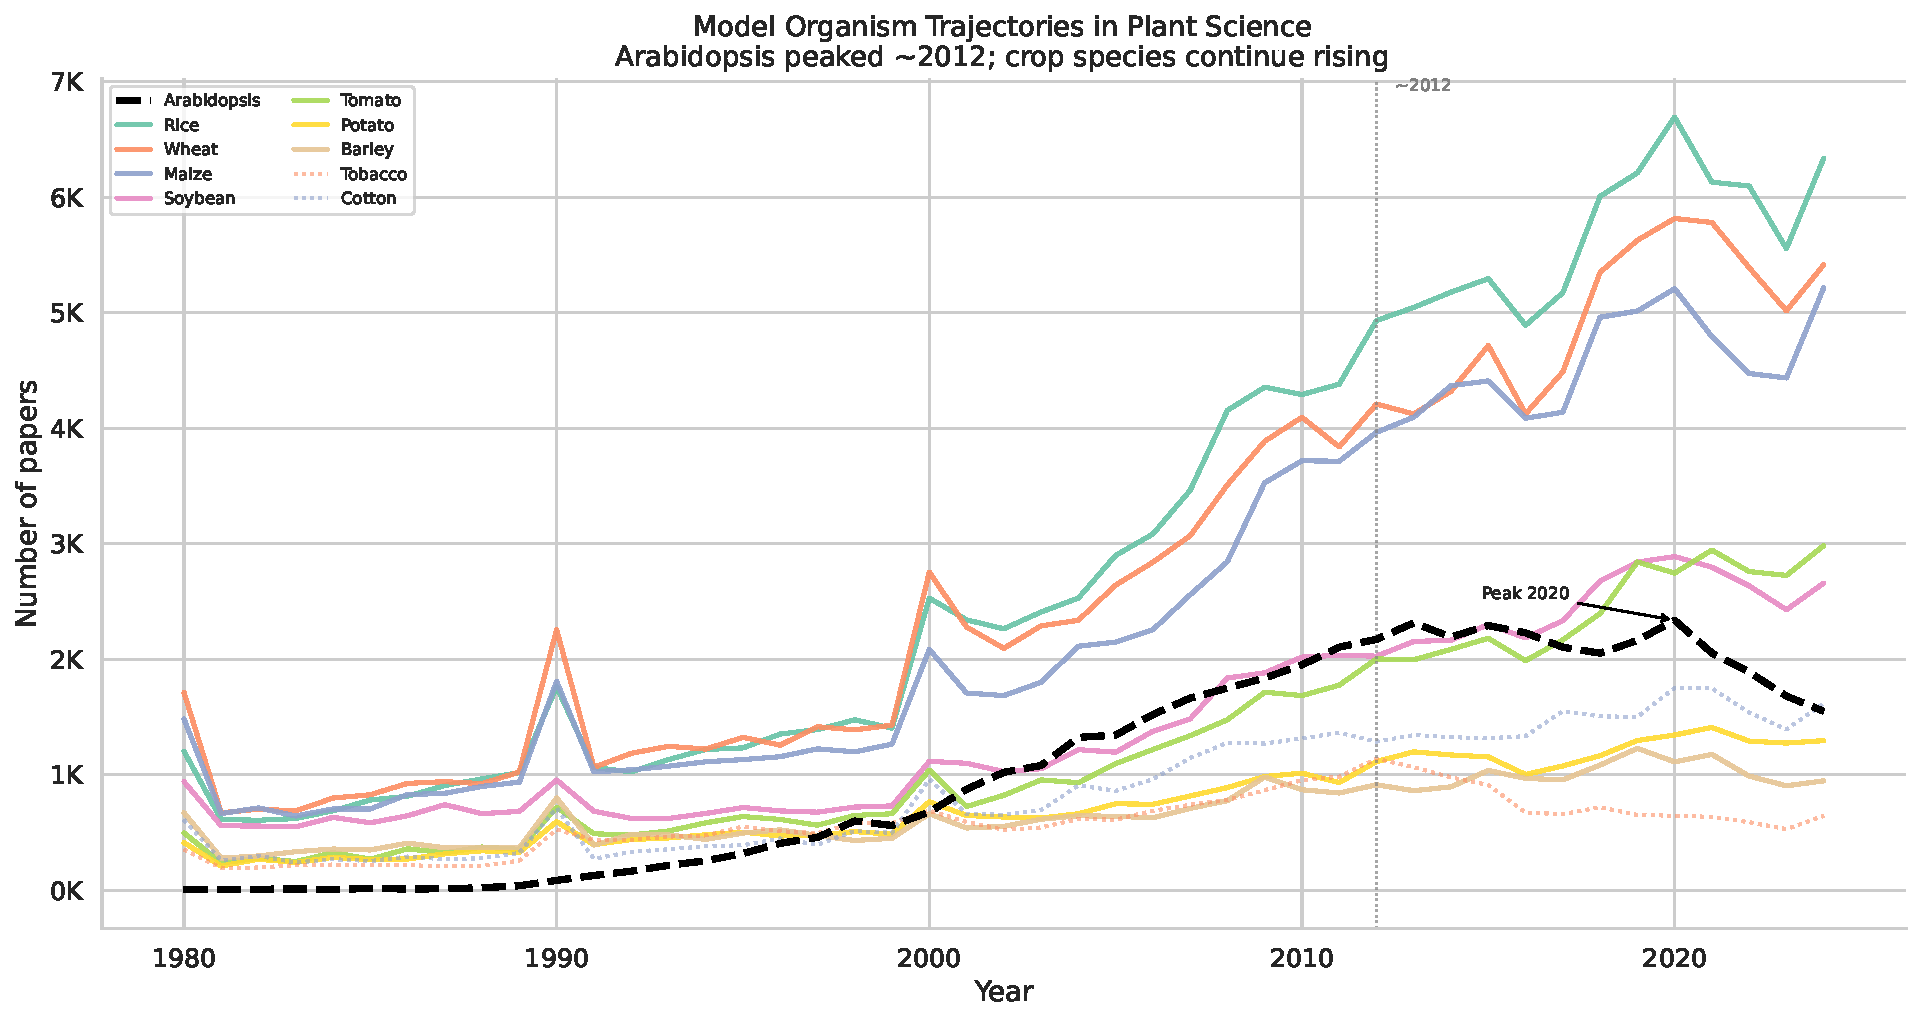
\includegraphics[width=0.72\textwidth]{FA2_model_organisms}
  \caption{\textbf{Model organism decline and crop species ascent.}
    Relative publication share (as percentage of annual plant science output)
    for \textit{Arabidopsis thaliana} (red), rice (blue), wheat (green), and
    maize (orange), 1990--2024.
    Vertical dashed line marks 2012, the year of peak
    \textit{Arabidopsis} relative share (see Discussion for the
    qualitative-nexus interpretation; the logistic growth inflection
    at 2006 is shown in Fig.~\ref{fig:FA1}).
    Secondary $y$-axis (right) shows absolute annual publication counts for
    \textit{Arabidopsis} to illustrate that relative decline precedes
    absolute decline.}
  \label{fig:FA2}
\end{figure}

% M2: Arabidopsis versus crops head-to-head share comparison
\begin{figure}[H]
  \centering
  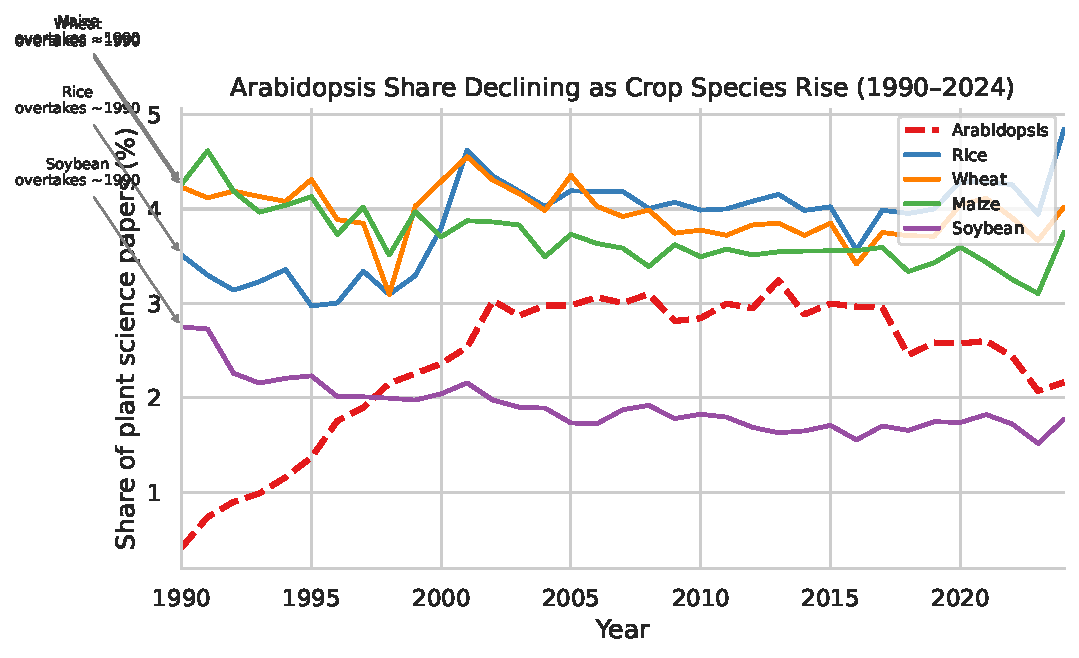
\includegraphics[width=0.72\textwidth]{M2_arabidopsis_vs_crops}
  \caption{\textbf{Arabidopsis versus crop species: head-to-head share
    comparison.}
    Direct comparison of \textit{Arabidopsis} (red) against the combined
    rice + wheat + maize share (blue), normalised to organism-specific papers
    only.
    The crossover point marks the transition from model-organism to crop-centred
    output majority.}
  \label{fig:M2}
\end{figure}

% M3: Applied versus fundamental paradigm by organism
\begin{figure}[H]
  \centering
  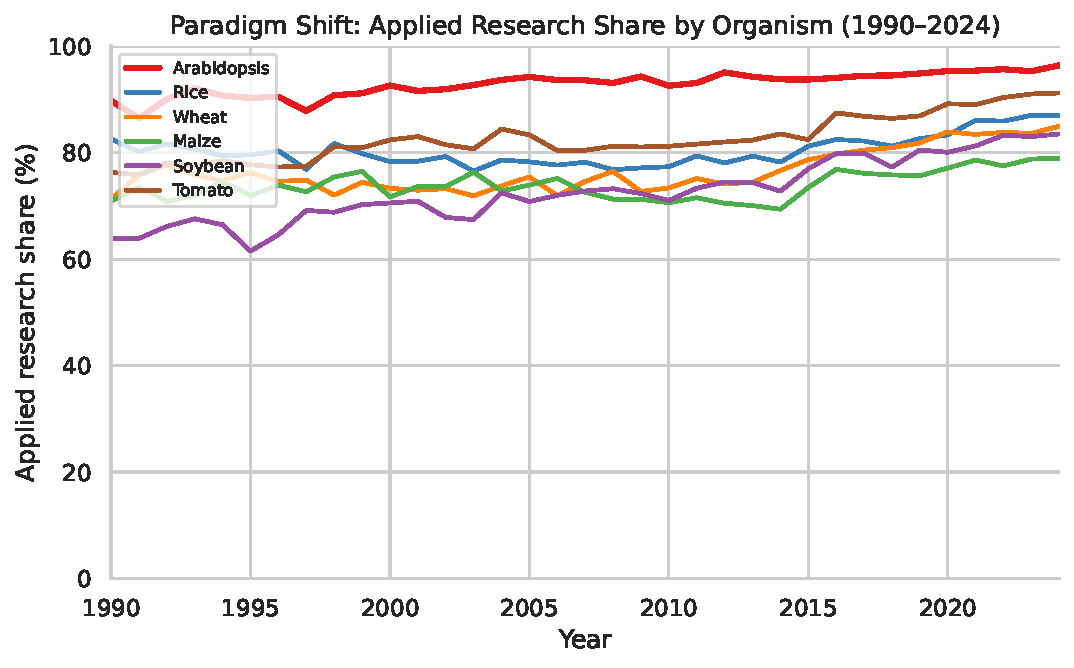
\includegraphics[width=0.72\textwidth]{M3_paradigm_shift}
  \caption{\textbf{Applied versus fundamental paradigm by organism.}
    Stacked bar chart of paradigm classification for each organism category.
    The field-wide applied share is 80\%; \textit{Arabidopsis} (95.6\%) is the
    most applied organism.
    Chi-square test: $\chi^2 = 12{,}361$, $df = 9$, $p \approx 0$.}
  \label{fig:M3}
\end{figure}

% M8: CRISPR-Cas9 adoption curves by organism
\begin{figure}[H]
  \centering
  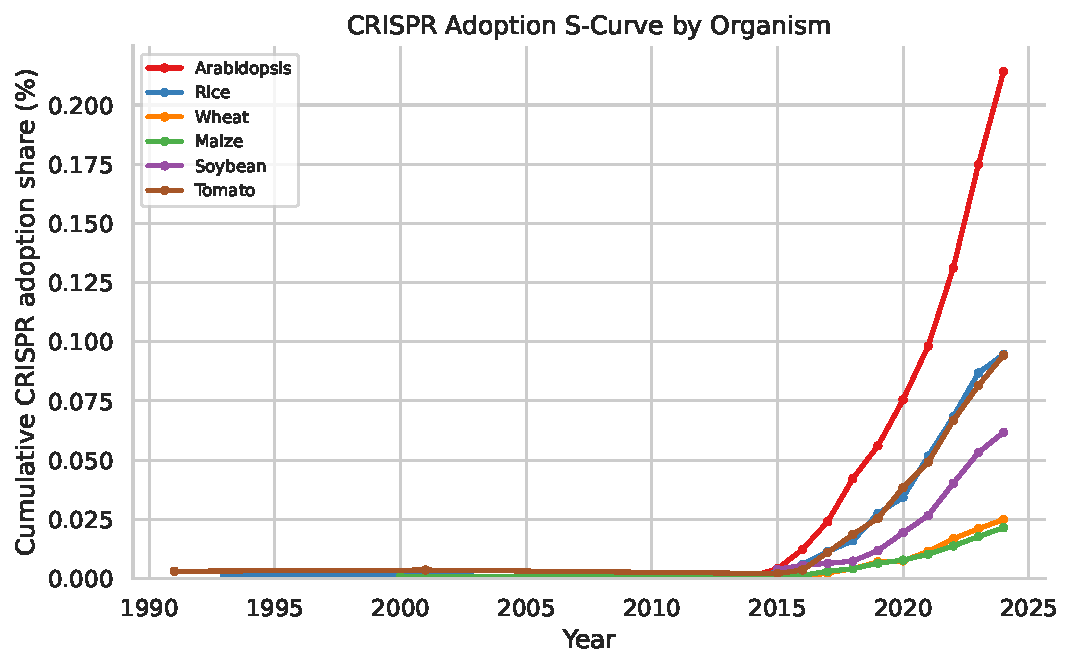
\includegraphics[width=0.72\textwidth]{M8_crispr_adoption}
  \caption{\textbf{CRISPR-Cas9 adoption curves by organism.}
    Annual CRISPR publication share for each organism category, 2012--2024.
    \textit{Arabidopsis} (red), rice (blue), and wheat (green) lead adoption;
    maize (orange) lags by approximately one year.
    Fitted logistic S-curves are shown as solid lines.}
  \label{fig:M8}
\end{figure}

% M4: Topic landscape — 30 macro-themes from BERTopic
\begin{figure}[H]
  \centering
  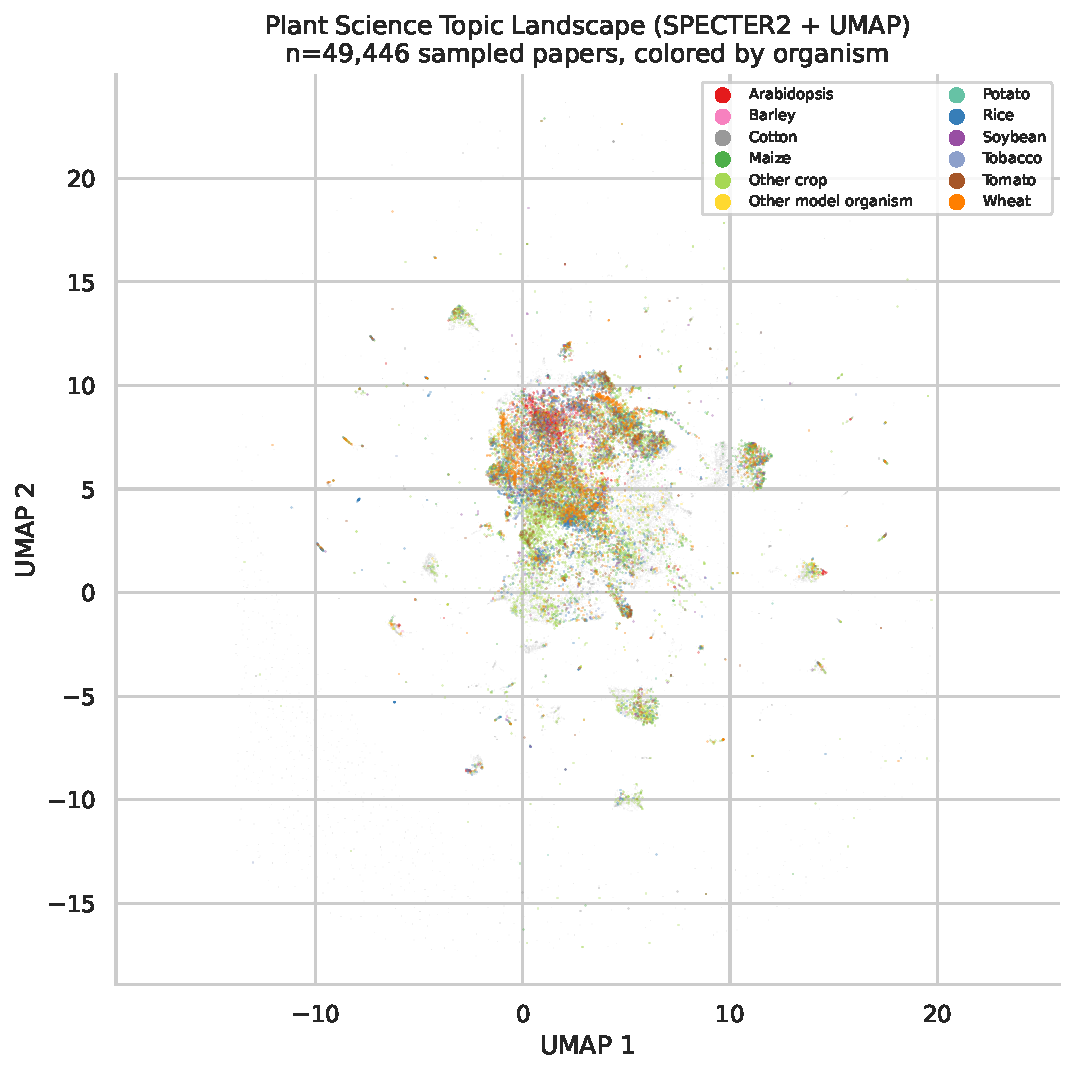
\includegraphics[width=0.52\textwidth]{M4_topic_landscape}
  \caption{\textbf{Topic landscape of plant science (SPECTER2 + UMAP).}
    UMAP projection of SPECTER2 embeddings for a sample of $n = 49{,}446$
    classified papers, coloured by organism category
    (\textit{Arabidopsis}, barley, cotton, maize, rice, soybean, tomato,
    tobacco, potato, wheat, other crop, other model organism; see
    legend). The 30 macro-themes obtained from BERTopic modelling of
    the full 1{,}632 fine-grained topics are described in the main
    text and visualised by their temporal trajectories in
    Fig.~\ref{fig:M5}.}
  \label{fig:M4}
\end{figure}

% M5: Topic evolution heatmap (1990–2024)
\begin{figure}[H]
  \centering
  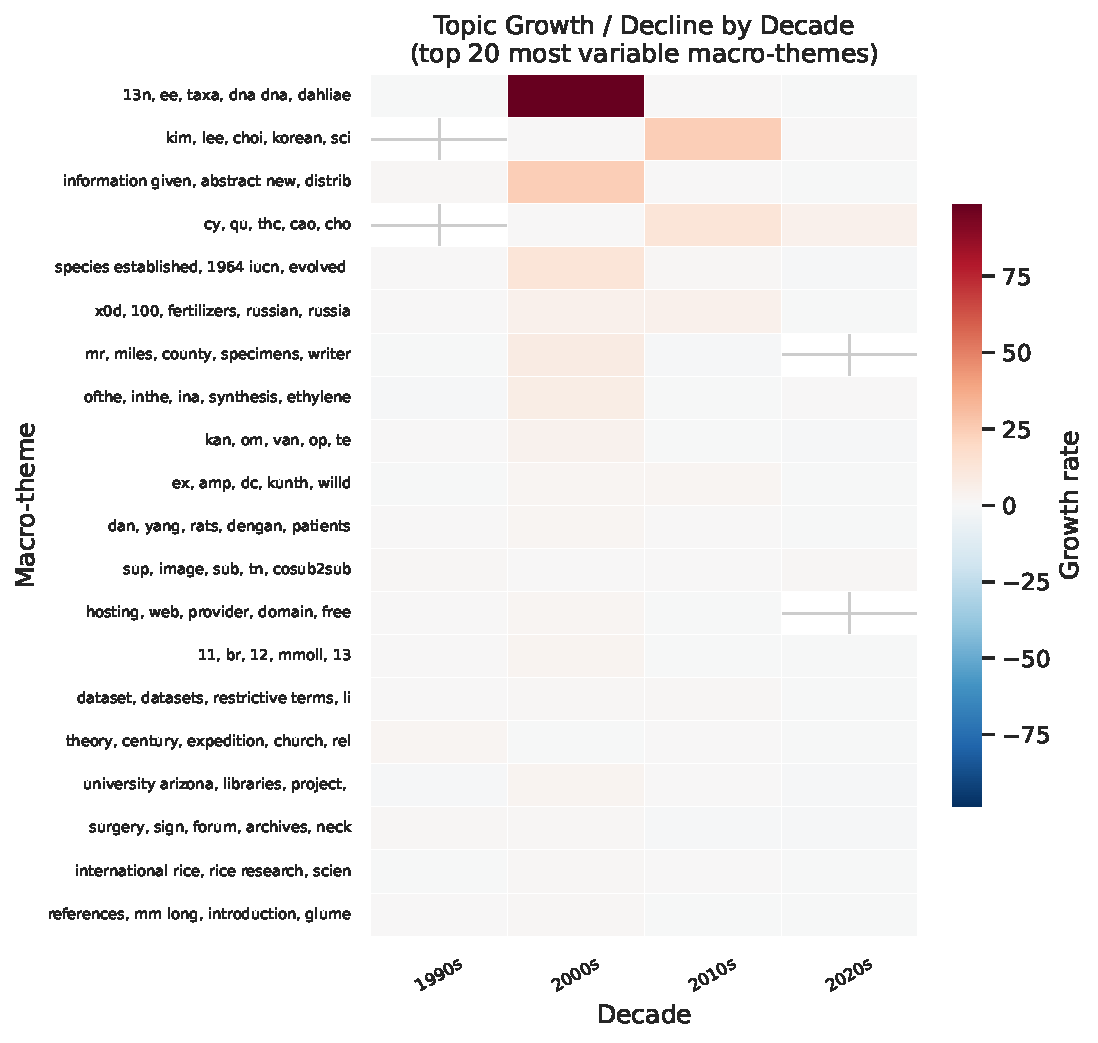
\includegraphics[width=0.60\textwidth]{M5_topic_evolution_heatmap}
  \caption{\textbf{Macro-theme growth/decline by decade (top 20 most
    variable macro-themes).}
    Heatmap of decadal growth rate for the 20 macro-themes with
    largest share change across 1990s--2020s.
    Cell colour gives the percentage-point change in publication
    share per decade (red = gaining share, blue = losing share).
    Row labels are the top BERTopic terms for each macro-theme
    (space-limited raw tokens; human-interpretable theme names given
    in main text). Across the 30 macro-themes (not all shown),
    Shannon entropy of the distribution has declined from
    1.82 bits (1990s mean) to 1.14 bits (2020s mean), indicating
    concentration of the research agenda.}
  \label{fig:M5}
\end{figure}

% M6: Organism-topic enrichment matrix
\begin{figure}[H]
  \centering
  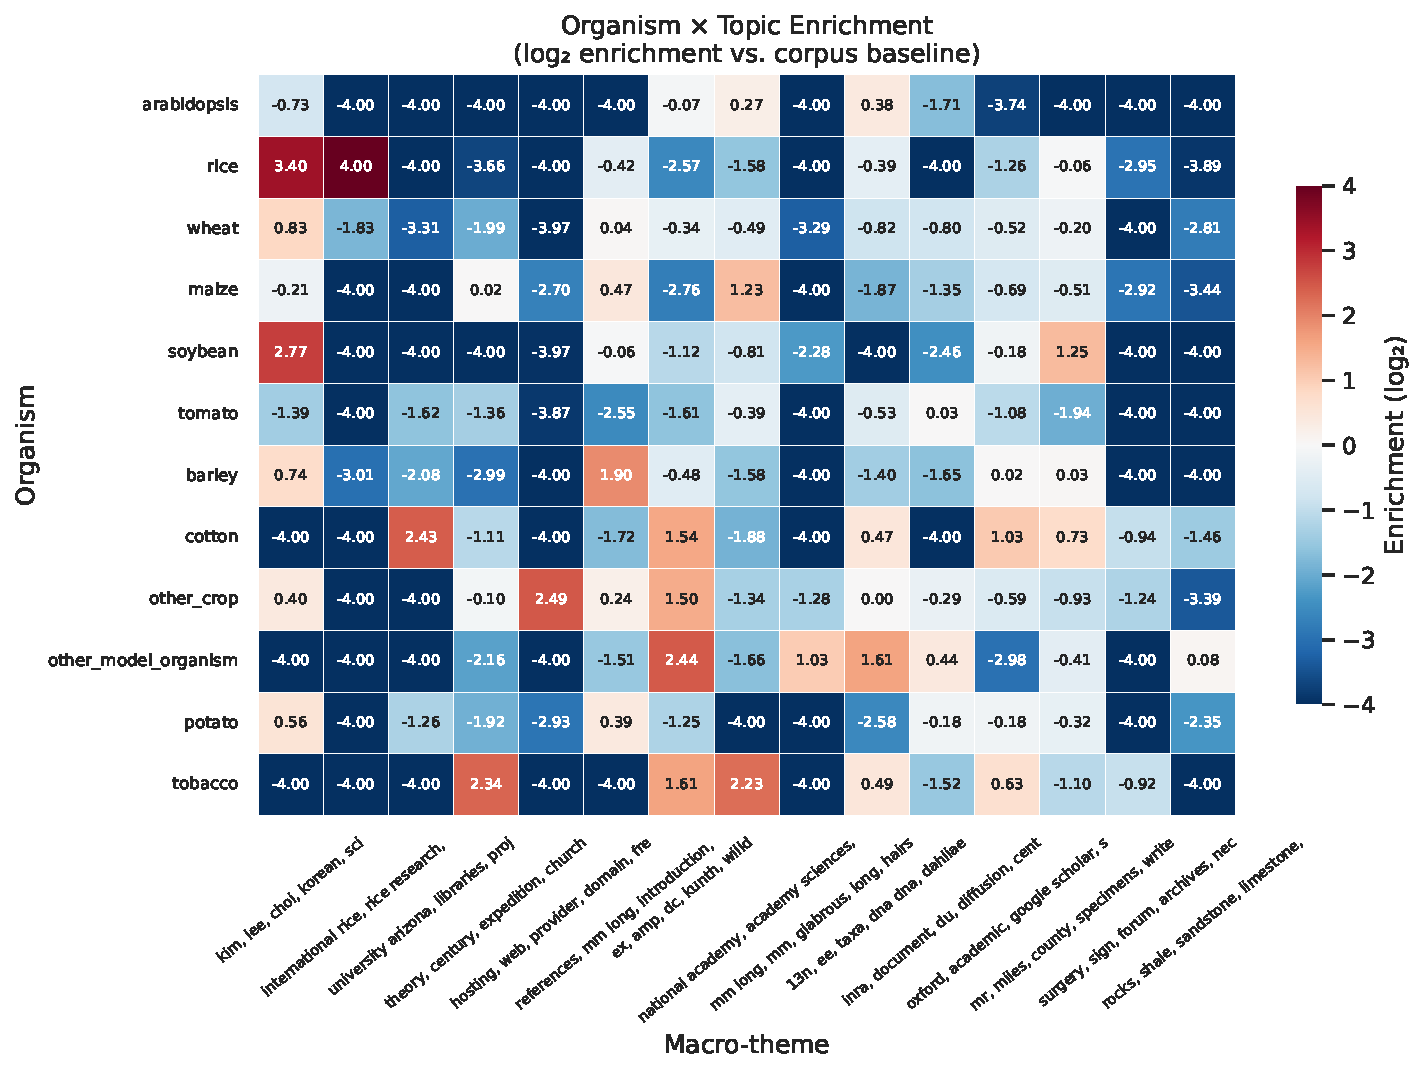
\includegraphics[width=0.72\textwidth]{M6_organism_topic_enrichment}
  \caption{\textbf{Organism-topic enrichment matrix.}
    Log-odds enrichment of each organism category for each macro-theme,
    relative to the field baseline.
    Significant enrichments ($p < 0.01$ after Bonferroni correction) are
    indicated by filled cells.}
  \label{fig:M6}
\end{figure}

% M7: Semantic drift — cosine distance of organism centroids from Arabidopsis
\begin{figure}[H]
  \centering
  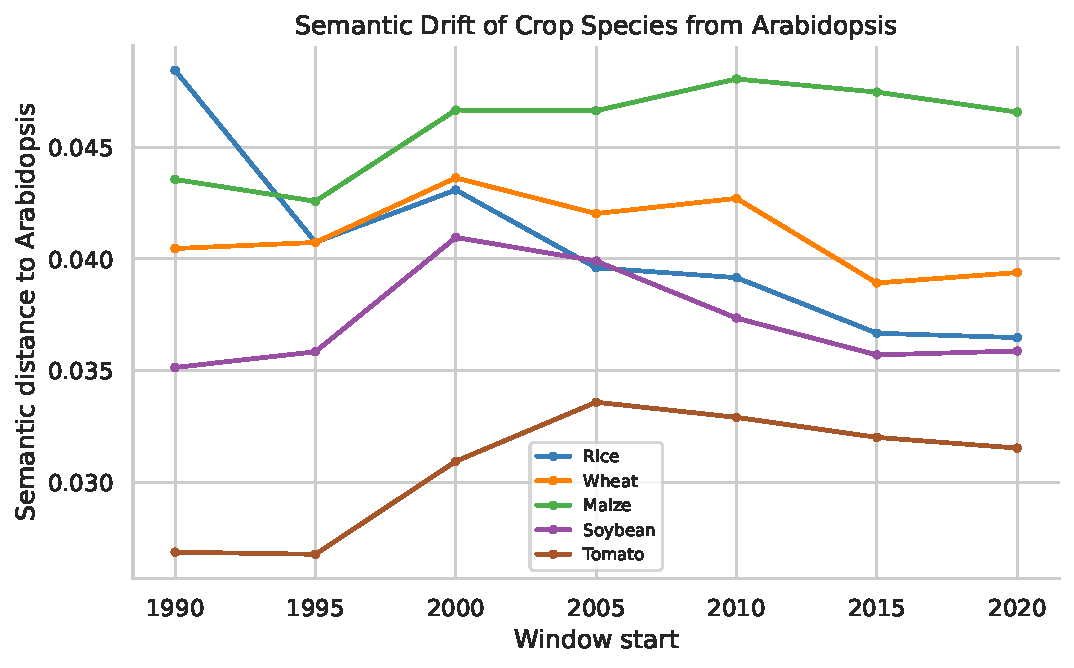
\includegraphics[width=0.72\textwidth]{M7_semantic_drift}
  \caption{\textbf{Semantic drift: cosine distance of organism centroids
    from \textit{Arabidopsis} (SPECTER2 embeddings).}
    Lower values indicate greater conceptual similarity to
    \textit{Arabidopsis}.
    Cotton (olive) and rice (blue) show the strongest convergence over
    2010--2024.
    Shaded band: 95\% bootstrap confidence interval.}
  \label{fig:M7}
\end{figure}

% FA5: Six intellectual epochs defined by concept marriages
\begin{figure}[H]
  \centering
  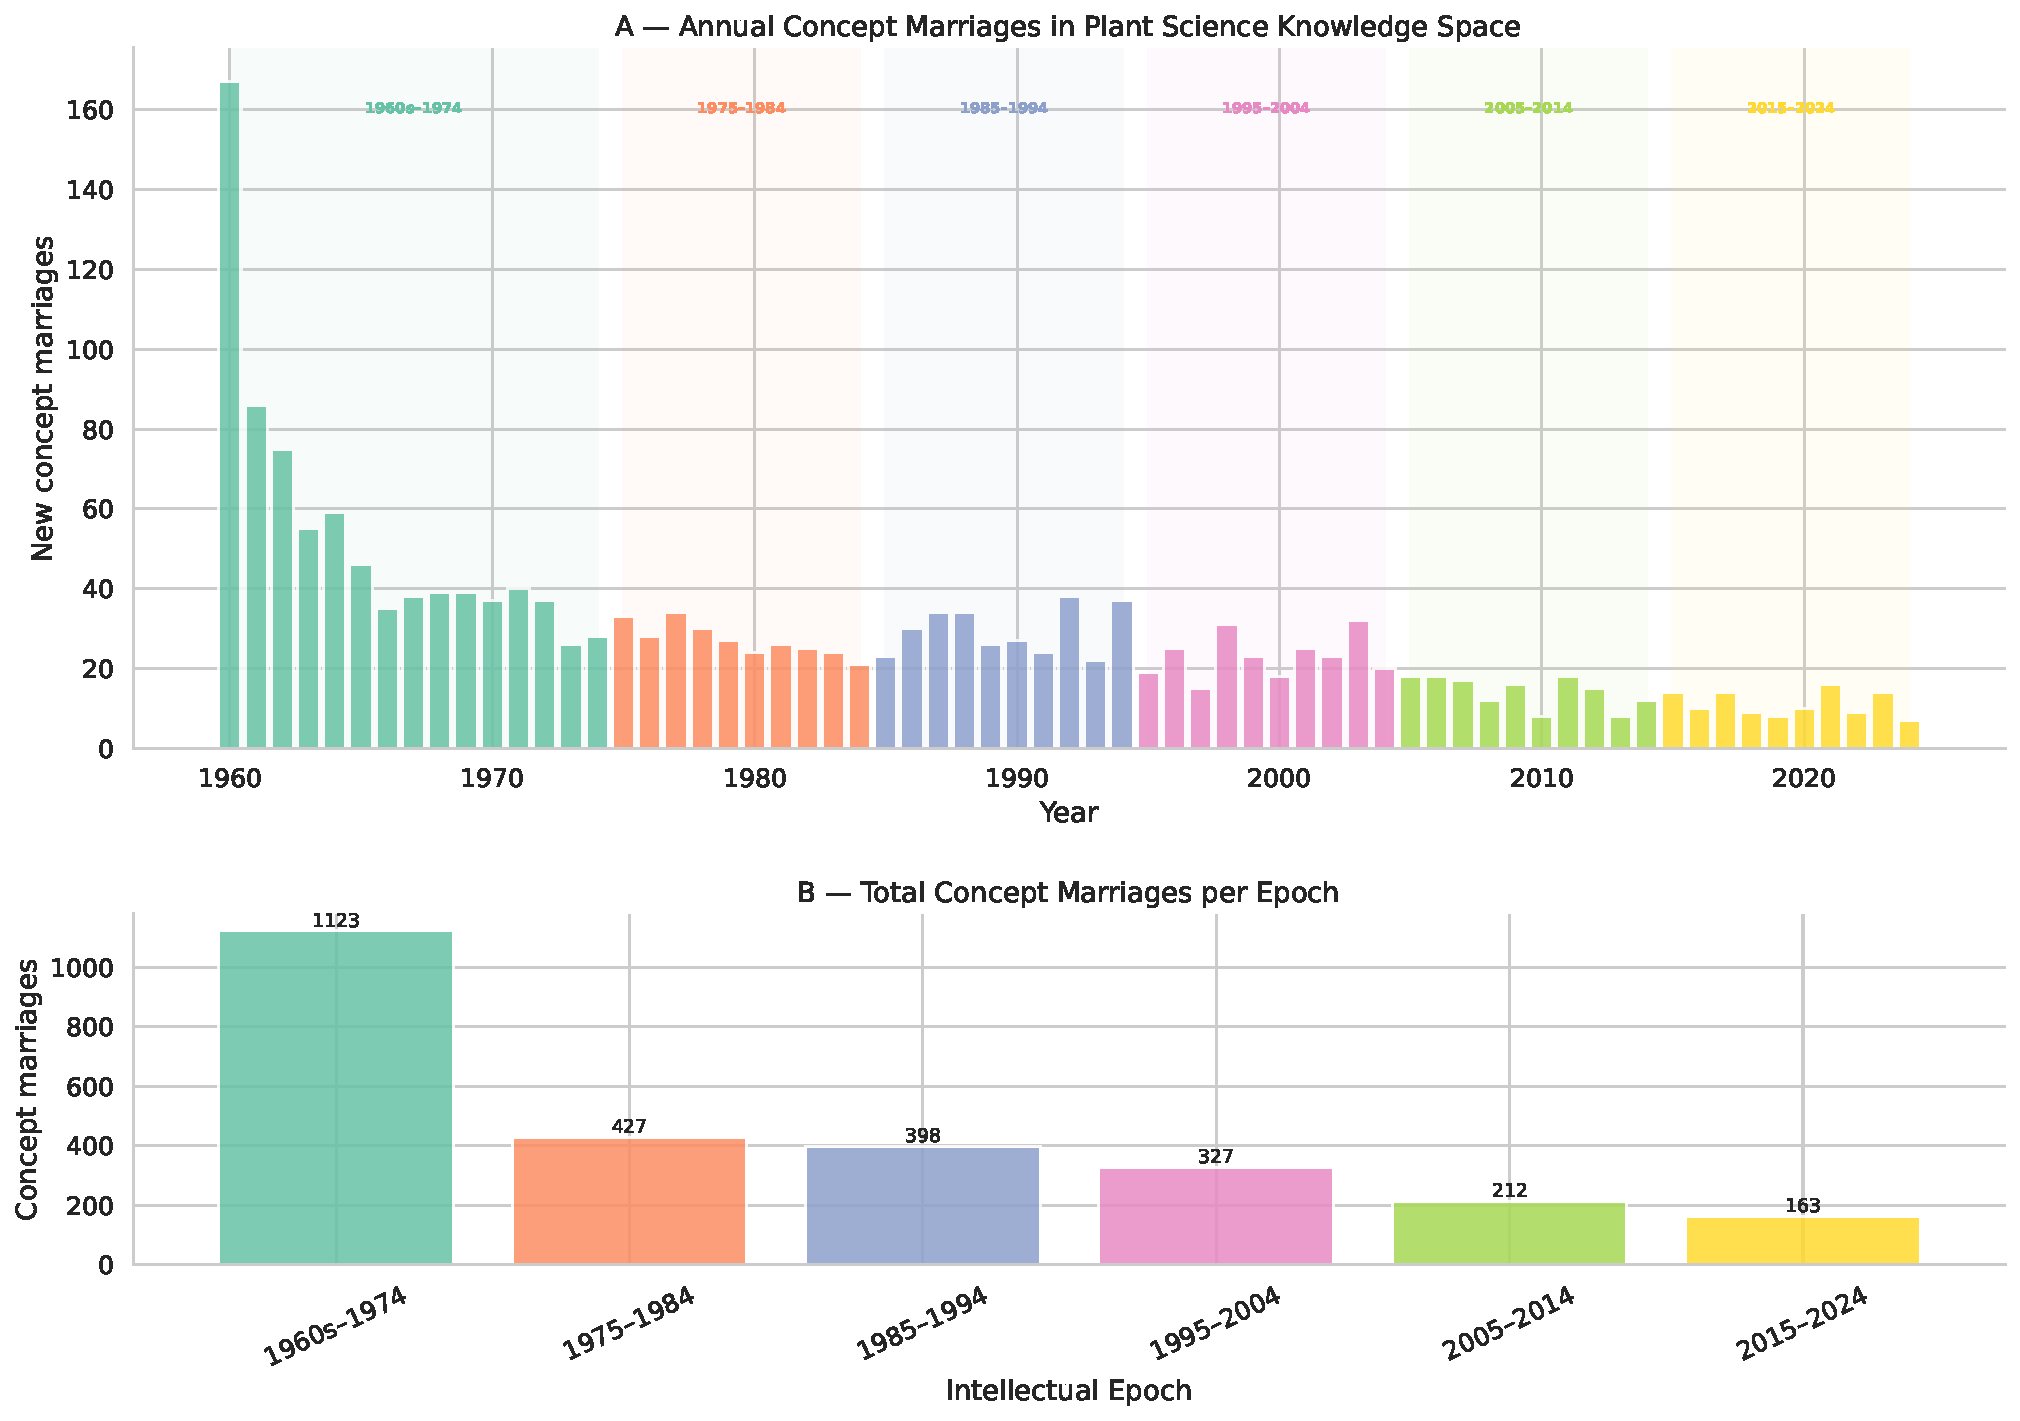
\includegraphics[width=0.60\textwidth]{FA5_concept_marriages}
  \caption{\textbf{Six intellectual epochs defined by concept marriages.}
    (\textbf{A}) Annual count of newly emerging concept marriages
    (new keyword pairs whose co-occurrence rose above the
    significance threshold) in the plant-science knowledge space,
    1960--2024. Background shading distinguishes the six epochs
    identified by hierarchical clustering of the concept
    co-occurrence matrix: 1960--1974, 1975--1984, 1985--1994,
    1995--2004, 2005--2014, 2015--2024.
    (\textbf{B}) Total concept marriages per epoch, showing a monotonic
    decline from 1{,}123 (1960--1974 cohort) to 163 (2015--2024
    cohort), consistent with a maturing knowledge space in which
    fewer genuinely novel keyword combinations emerge each year.
    The 2015--2024 epoch is dominated by crop-genomics and
    precision-breeding marriages (main text).}
  \label{fig:FA5}
\end{figure}

% End of Extended Data; subsequent SI figures will continue the ED counter,
% which is fine because SI figures use manually-labeled captions (see
% supplementary.tex "Supplementary Figure S1..." headings that don't rely
% on auto-numbering).


% ── Data Availability ─────────────────────────────────────────────────
\section*{Data Availability}
The OpenAlex and PubMed bibliographic records used in this study are
publicly available from \url{https://openalex.org} and
\url{https://pubmed.ncbi.nlm.nih.gov}, respectively.
The processed corpus (deduplicated DOI list, organism and paradigm
classification labels, BERTopic topic assignments, and derived
result tables) is archived at Zenodo:
\url{https://doi.org/10.5281/zenodo.21199139}.
FAO production statistics used for the research-attention gap analysis
are available from \url{https://www.fao.org/faostat/}.

% ── Code Availability ─────────────────────────────────────────────────
\section*{Code Availability}
All analysis code, SLURM batch scripts, and figure generation scripts
are available at
\url{https://github.com/ehsanestaji/plant-science-paradigm-shift}
under the MIT licence.
The GPU-accelerated embedding and classification pipeline requires
PyTorch~2.7.1 and an NVIDIA A100 GPU; all other analysis scripts are
CPU-only and can be run on a standard workstation with 64\,GB RAM.
A reproducible environment specification (\texttt{requirements.txt} and
\texttt{environment.yml}) is included in the repository root.

% ── Author Contributions ──────────────────────────────────────────────
\section*{Author Contributions}
E.E.\ and J.-F.M.\ conceived the study. E.E.\ designed and performed all
analyses and wrote the manuscript. J.-F.M.\ contributed critical revisions
to the manuscript. All authors read and approved the final version.

% ── Competing Interests ───────────────────────────────────────────────
\section*{Competing Interests}
The authors declare no competing interests.

% ── Funding ───────────────────────────────────────────────────────────
\section*{Funding}
This work was partially supported by the Wallenberg Initiatives in Forest
Research (WIFORCE), funded by the Knut and Alice Wallenberg Foundation.

% ── Acknowledgments ───────────────────────────────────────────────────
\section*{Acknowledgments}
We thank OpenAlex, PubMed, and FAO for openly releasing the
bibliographic and agricultural-production data on which this study
depends. Computational resources for the GPU-accelerated embedding
and classification pipeline were provided by HPC2N (Umeå) via
project \texttt{hpc2n2025-278}; post-hoc robustness and insights
analyses were run on local Apple Silicon workstations. We thank the
\texttt{leidenalg}, \texttt{igraph}, \texttt{DuckDB}, \texttt{BERTopic},
and \texttt{SPECTER2} open-source maintainers whose tools underpin
the analyses reported here.

% ── References ────────────────────────────────────────────────────────
\bibliographystyle{naturemag}
\bibliography{references}

% ── Index of display items and supplementary materials ────────────────
% (placed after the reference list, before the Supplementary Information)
\clearpage
% ============================================================
%  Paper A — Index of display items and supplementary materials
%  Numbers are pulled via \ref so they stay in sync with the
%  actual figure/table/note counters.
% ============================================================

\section*{List of Main-Text Display Items}

\subsection*{Main-text figures}
\begin{itemize}\setlength{\itemsep}{2pt}
  \item \textbf{Figure~\ref{fig:FA1}.} Logistic growth plateau in plant
        science publications.
  \item \textbf{Figure~\ref{fig:M9}.} \textit{Arabidopsis} consolidates as
        crop science's methodological substrate (instrumentalization ratio
        and reverse-translation lag).
  \item \textbf{Figure~\ref{fig:M1}.} Organism-share time series from
        zero-shot classification (2.77 million papers).
  \item \textbf{Figure~\ref{fig:FA3}.} Sleeping-beauty awakenings cluster in
        2019--2022.
  \item \textbf{Figure~\ref{fig:FA4}.} Method-diffusion S-curves in plant
        science.
  \item \textbf{Figure~\ref{fig:FA6}.} The orphan-organism
        research-attention gap.
\end{itemize}

\subsection*{Main-text tables}
None. The main text contains no tables; all tabular data are provided as
Supplementary Tables (below).

\subsection*{Extended Data figures}
\begin{itemize}\setlength{\itemsep}{2pt}
  \item \textbf{Extended Data Fig.~\ref{fig:FA2}.} Model-organism decline and
        crop-species ascent.
  \item \textbf{Extended Data Fig.~\ref{fig:M2}.} \textit{Arabidopsis} versus
        crop species --- head-to-head share comparison.
  \item \textbf{Extended Data Fig.~\ref{fig:M3}.} Applied versus fundamental
        paradigm by organism.
  \item \textbf{Extended Data Fig.~\ref{fig:M8}.} CRISPR-Cas9 adoption curves
        by organism.
  \item \textbf{Extended Data Fig.~\ref{fig:M4}.} Topic landscape of plant
        science (SPECTER2 + UMAP).
  \item \textbf{Extended Data Fig.~\ref{fig:M5}.} Macro-theme growth/decline
        by decade.
  \item \textbf{Extended Data Fig.~\ref{fig:M6}.} Organism--topic enrichment
        matrix.
  \item \textbf{Extended Data Fig.~\ref{fig:M7}.} Semantic drift of organism
        centroids toward \textit{Arabidopsis}.
  \item \textbf{Extended Data Fig.~\ref{fig:FA5}.} Six intellectual epochs
        defined by concept marriages.
\end{itemize}

\clearpage
\section*{List of Supplementary Materials}

\subsection*{Supplementary figures}
\begin{itemize}\setlength{\itemsep}{2pt}
  \item \textbf{Supplementary Fig.~\ref{fig:S1}.} Annual growth rates by
        organism (classified corpus).
  \item \textbf{Supplementary Fig.~\ref{fig:S2}.} Citation impact by paradigm
        and organism.
  \item \textbf{Supplementary Fig.~\ref{fig:S3}.} Shannon entropy of the
        macro-theme distribution by year.
  \item \textbf{Supplementary Fig.~\ref{fig:S6}.} CD disruption index by
        organism.
  \item \textbf{Supplementary Fig.~\ref{fig:S9}.} Cross-citation matrix
        between organism categories.
  \item \textbf{Supplementary Fig.~\ref{fig:S10}.} International collaboration
        rate by organism.
  \item \textbf{Supplementary Fig.~\ref{fig:s-temporal-placebo}.} Temporal
        placebo test.
  \item \textbf{Supplementary Fig.~\ref{fig:s-growth-aic}.} Growth-model
        comparison (logistic, Gompertz, Richards).
  \item \textbf{Supplementary Fig.~\ref{fig:s-climate-shocks}.} Pooled
        climate-event publication response.
  \item \textbf{Supplementary Fig.~\ref{fig:s-bridge-impact}.} Mean
        citations-per-paper by paradigm class.
  \item \textbf{Supplementary Fig.~\ref{fig:s-paradigm-alignment}.} Paradigm
        alignment in the coauthor graph.
  \item \textbf{Supplementary Fig.~\ref{fig:s-jaccard-over-time}.} Jaccard
        overlap of consecutive-window top-100 reference sets.
  \item \textbf{Supplementary Fig.~\ref{fig:s-reference-half-life}.} Reference
        half-life.
  \item \textbf{Supplementary Fig.~\ref{fig:s-composition-over-time}.}
        Top-100 canon composition, 1995--2024.
  \item \textbf{Supplementary Fig.~\ref{fig:s-top-substitution-pair}.} Top
        anti-correlated (fallen $\times$ riser) citation trajectories.
\end{itemize}

\subsection*{Supplementary tables}
\begin{itemize}\setlength{\itemsep}{2pt}
  \item \textbf{Supplementary Table~\ref{tab:S1}.} Crops ranked by
        research-attention gap.
  \item \textbf{Supplementary Table~\ref{tab:S2}.} Top sleeping-beauty papers
        by $B$-index.
  \item \textbf{Supplementary Table~\ref{tab:S3}.} Logistic diffusion-model
        parameters for methodologies.
  \item \textbf{Supplementary Table~\ref{tab:S7}.} Three-way comparison of
        sigmoidal growth-model fits.
  \item \textbf{Supplementary Table~\ref{tab:S11-risers}.} Top-5 risers in the
        2020--24 top-100 reference list.
  \item \textbf{Supplementary Table~\ref{tab:S11-fallen}.} Top-5 fallen
        classics.
  \item \textbf{Supplementary Table~\ref{tab:S11-substitution}.} Top
        anti-correlated (fallen $\times$ riser) reference pairs.
\end{itemize}

\subsection*{Supplementary notes}
\begin{itemize}\setlength{\itemsep}{2pt}
  \item \textbf{Supplementary Note~\ref{sec:temporal-placebo}.} Temporal
        placebo test (reorganization signal).
  \item \textbf{Supplementary Note~\ref{sec:growth-model-aic}.} Growth-model
        selection --- logistic vs Gompertz vs Richards.
  \item \textbf{Supplementary Note~\ref{sec:climate-shocks}.} Climate-shock
        event study (pooled difference-in-differences).
  \item \textbf{Supplementary Note~\ref{sec:bridge-scientists}.}
        Paradigm-bridging authors --- pre-registered matched-impact analysis.
  \item \textbf{Supplementary Note~\ref{sec:coauthor-alignment}.} Coauthor
        paradigm alignment over time (network-only).
  \item \textbf{Supplementary Note~\ref{sec:canon-churn}.} Canon churn ---
        the plant-science reading list, 1995--2024 (incl.\ canon substitution).
\end{itemize}


% ── Supplementary Information (placed at the end of the document) ──────
\clearpage
\appendix
\section*{Supplementary Information}
% ============================================================
%  Paper A — Supplementary Information
% ============================================================

% Reset figure and table counters + prefixes so SI elements are
% auto-numbered "Supplementary Figure S1, S2, ..." and
% "Supplementary Table S1, S2, ...". Without these the ED figure counter
% would bleed through (captions would read "Extended Data Fig. 10, 11,
% ...") and the global table counter would give "Table 1, 2, 3" on our
% SI tables.
\setcounter{figure}{0}
\setcounter{table}{0}
\renewcommand{\figurename}{Supplementary Figure}
\renewcommand{\tablename}{Supplementary Table}
\renewcommand{\thefigure}{S\arabic{figure}}
\renewcommand{\thetable}{S\arabic{table}}

% Auto-numbered Supplementary Notes (narrative analyses), numbered 1..N
% in order of appearance and cross-referenced via \ref. Figure/table-holder
% subsections keep descriptive headers; they are identified by their
% Supplementary Figure/Table number.
\newcounter{snote}
\newcommand{\suppnote}[2]{%
  \refstepcounter{snote}%
  \subsection*{Supplementary Note~\arabic{snote}: #1}%
  \label{#2}%
}

% ── GPU-derived supplementary figures ──────────────────────────────────

\subsection*{Organism growth rates (classified corpus)}

\begin{figure}[H]
  \centering
  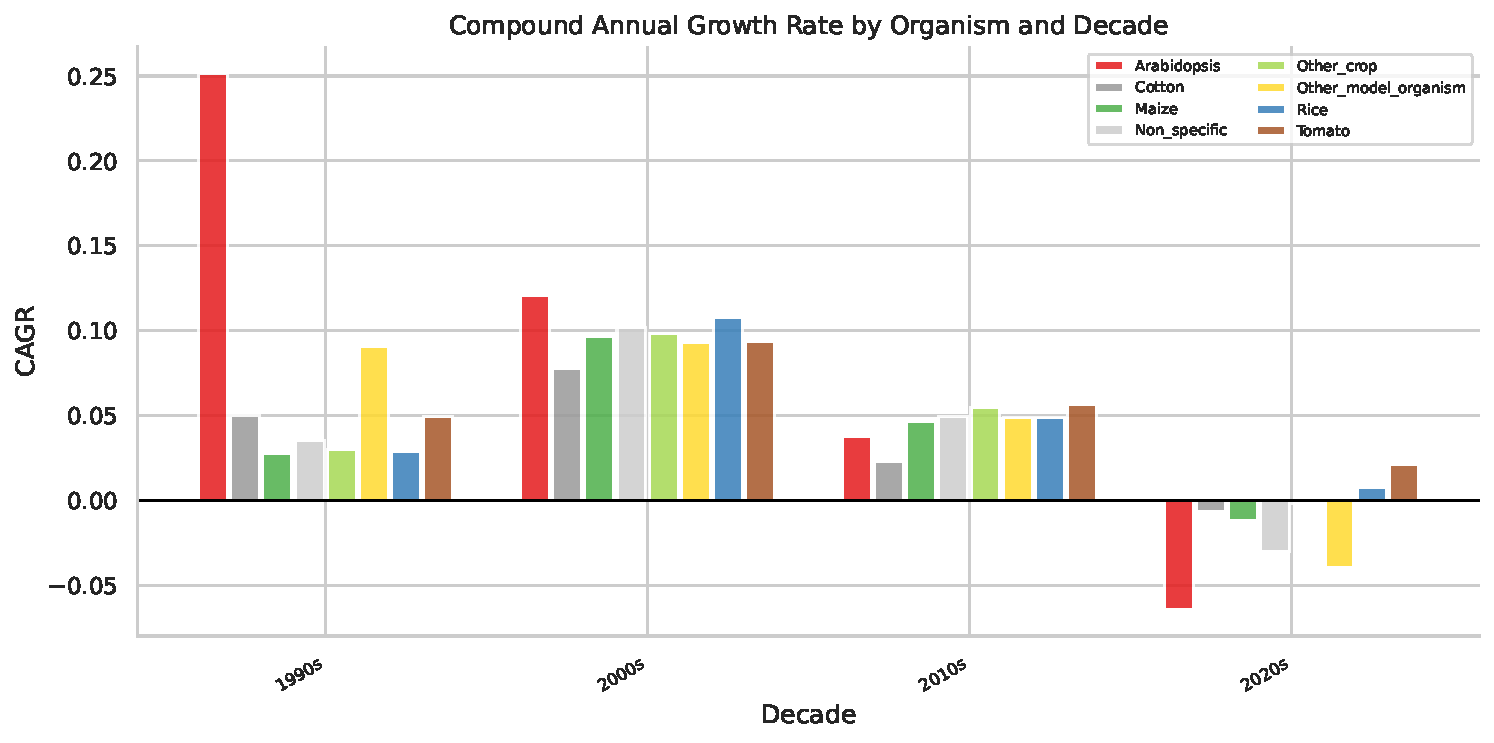
\includegraphics[width=0.72\textwidth]{S1_growth_rates}
  \caption{\textbf{Annual growth rates by organism (zero-shot classified corpus,
    2.77 million papers).}
    CAGR computed over the 2010s and 2020s for each organism category.
    Rice leads crop-organism growth in the 2010s (CAGR 4.9\%); most organism
    groups show slower or negative growth in the 2020s consistent with
    field-level plateau.}
  \label{fig:S1}
\end{figure}

\subsection*{Paradigm classification and citation impact}

\begin{figure}[H]
  \centering
  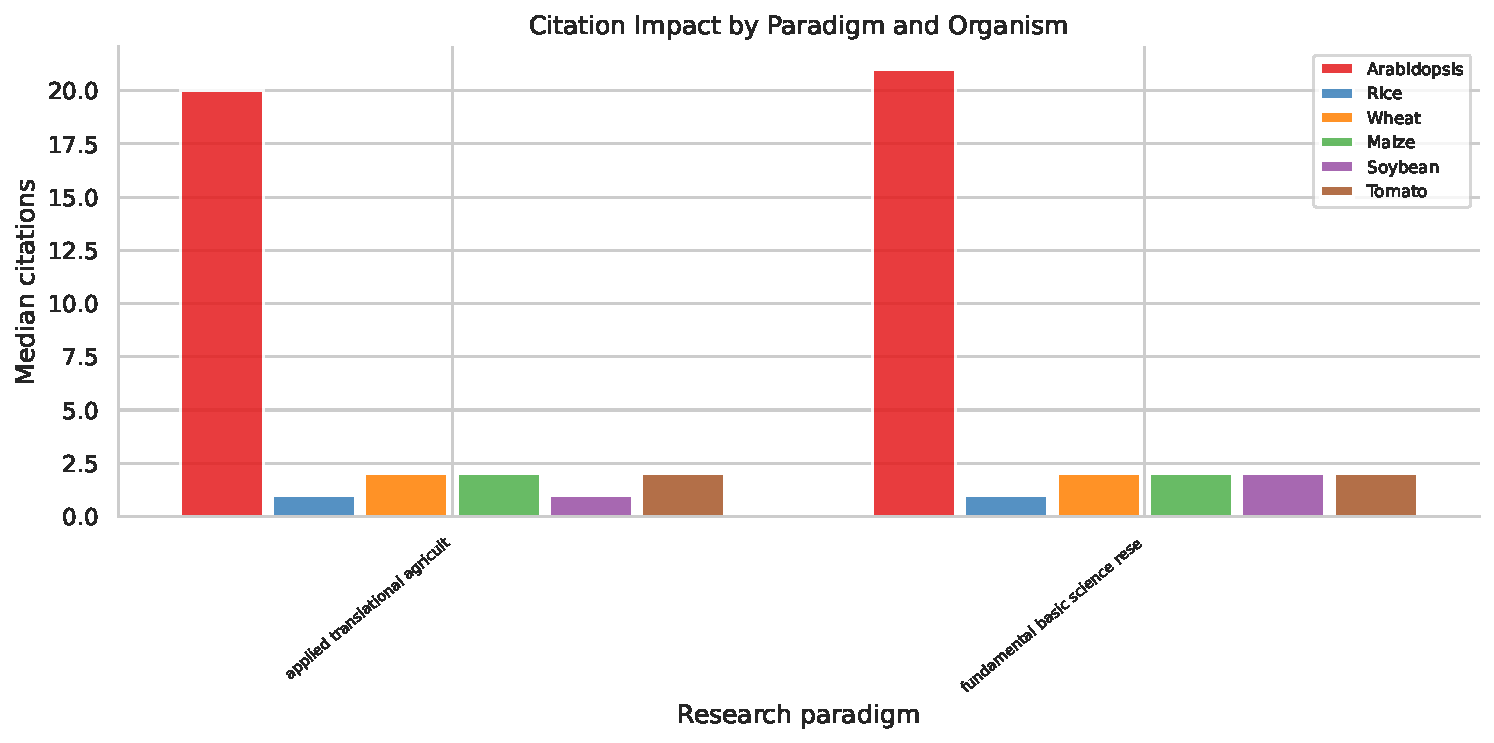
\includegraphics[width=0.72\textwidth]{S2_paradigm_citations}
  \caption{\textbf{Citation impact by paradigm and organism.}
    Box plots of five-year forward citation counts for applied versus fundamental
    papers, stratified by organism.
    Applied \textit{Arabidopsis} papers show the highest median citation counts;
    fundamental papers in crop organisms show high variance reflecting a small
    number of highly cited mechanistic studies.}
  \label{fig:S2}
\end{figure}

\subsection*{Topic diversity by year}

\begin{figure}[H]
  \centering
  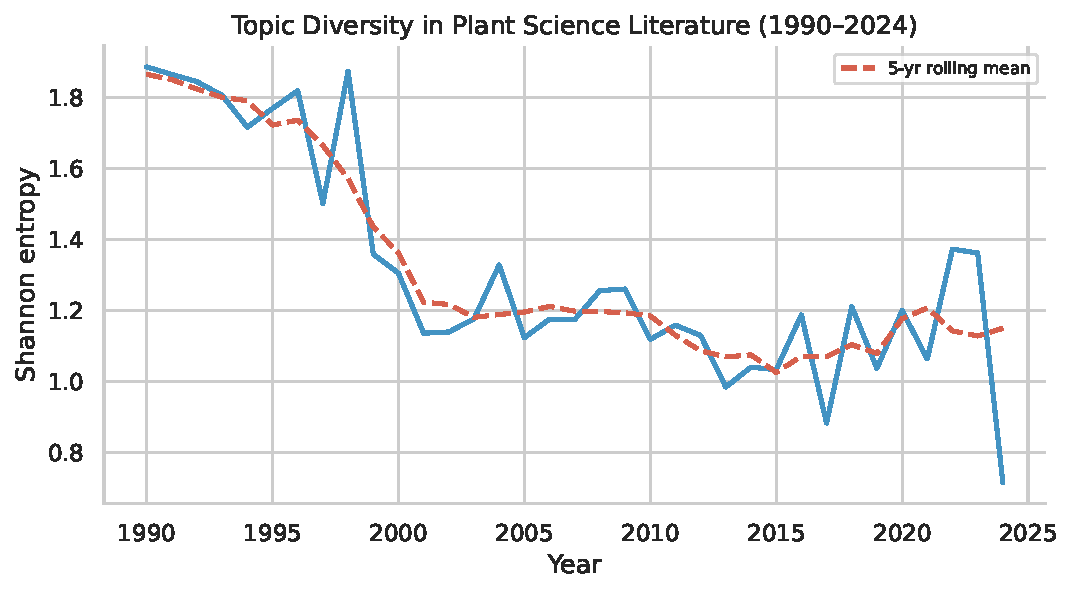
\includegraphics[width=0.72\textwidth]{S3_topic_diversity}
  \caption{\textbf{Shannon entropy of macro-theme distribution by year
    (1990--2024).}
    Entropy declined from 1.82 bits (1990s mean) to 1.14 bits (2020s mean),
    reflecting concentration of the research agenda around a smaller set of
    dominant themes.
    Shaded region: 95\% bootstrap confidence interval.}
  \label{fig:S3}
\end{figure}

\subsection*{Disruption index by organism}

\begin{figure}[H]
  \centering
  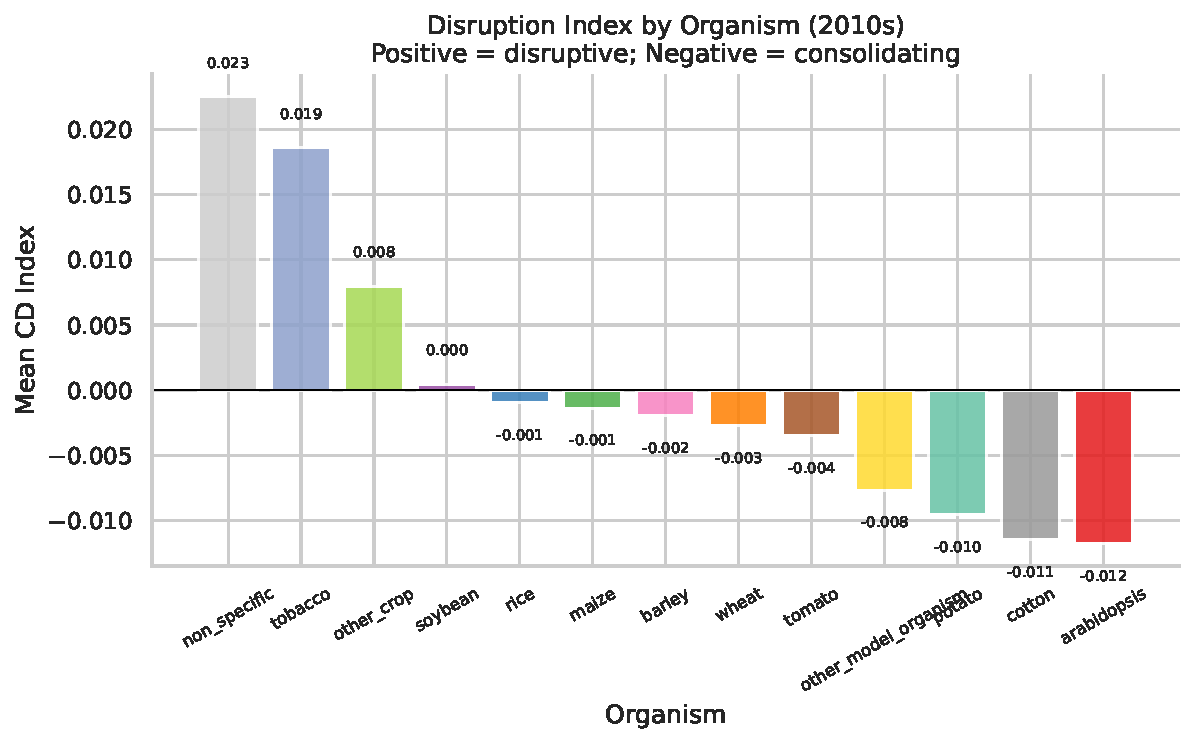
\includegraphics[width=0.72\textwidth]{S6_disruption_index}
  \caption{\textbf{CD disruption index by organism, decade resolution.}
    \textit{Arabidopsis} has the most negative mean CD index ($-0.001$),
    indicating consolidation; crop species (maize 0.095, soybean 0.102,
    cotton 0.099) are consistently more disruptive.
    Error bars: standard error of the mean across decades.
    Kruskal--Wallis test: $H = 12.9$, $p = 0.17$, $n_{\mathrm{groups}} = 10$.}
  \label{fig:S6}
\end{figure}

\subsection*{Cross-citation matrix between organism categories}

\begin{figure}[H]
  \centering
  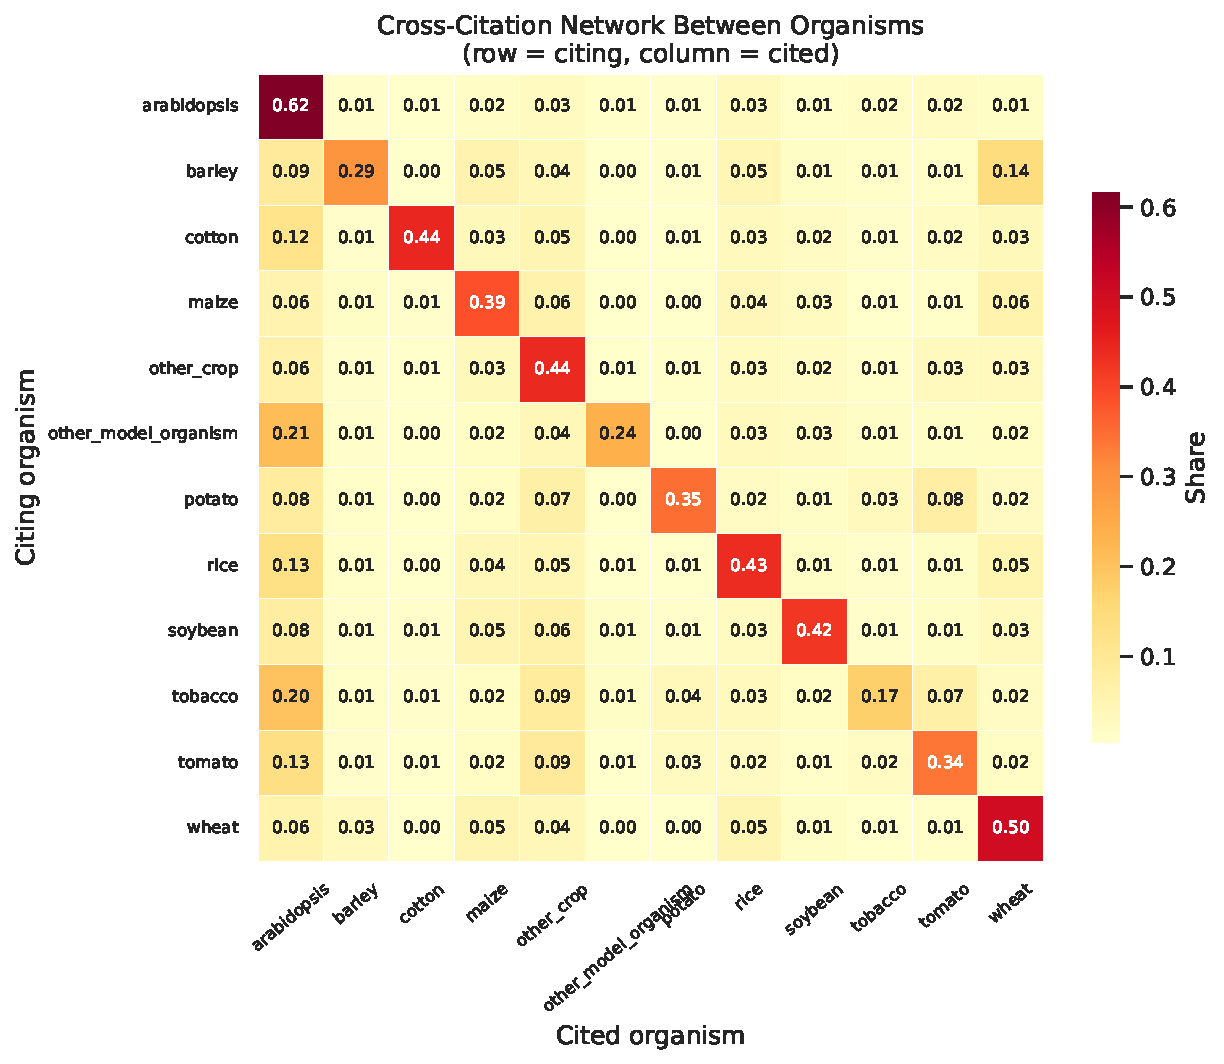
\includegraphics[width=0.72\textwidth]{S9_cross_citation}
  \caption{\textbf{Cross-citation matrix between organism categories
    (2020--2024).}
    Cell values give the fraction of citations from organism~$i$ (row) to
    papers in organism category~$j$ (column).
    \textit{Arabidopsis} has the highest self-citation rate (61.6\%);
    crop organisms cite \textit{Arabidopsis} at rates of 10--20\%,
    confirming continued intellectual dependence on the model organism.}
  \label{fig:S9}
\end{figure}

\subsection*{International collaboration by organism}

\begin{figure}[H]
  \centering
  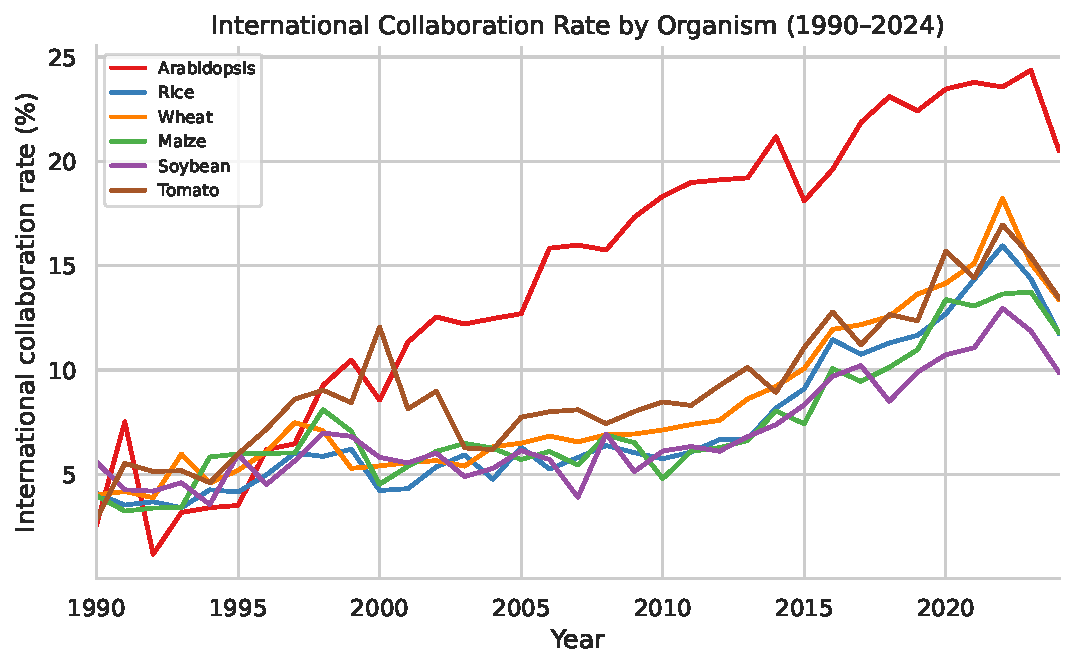
\includegraphics[width=0.72\textwidth]{S10_collaboration}
  \caption{\textbf{International collaboration rate by organism (2020--2024).}
    \textit{Arabidopsis} has the highest international collaboration rate
    (18.9\%), followed by other model organisms (16.2\%) and barley (16.1\%).
    Soybean (11.3\%) and non-specific papers (9.8\%) have the lowest rates.}
  \label{fig:S10}
\end{figure}

% ── Traditional supplementary tables ───────────────────────────────────

\subsection*{Orphan crops ranked by research-attention gap}

Plants are ranked by attention gap index (log$_2$ ratio of papers per trillion
kilocalories). Negative values indicate under-studied species relative to their
caloric importance. Data from FAO production statistics and OpenAlex corpus
(1900--2024).

\begin{table}[H]
\centering
\caption{Crops ranked by research-attention gap (most under-studied first).}
\label{tab:S1}
\begin{tabular}{rlrrrr}
\toprule
Rank & Crop & Publications & Production (Mt) & Papers/Mt & Attention gap \\
\midrule
1  & Sugarcane       & 30,220  & 1,900 & 15.9    & $-4.27$ \\
2  & Cassava         & 21,135  & 310   & 68.2    & $-2.17$ \\
3  & Maize           & 138,597 & 1,160 & 119.5   & $-1.36$ \\
4  & Potato          & 52,825  & 375   & 140.9   & $-1.12$ \\
5  & Wheat           & 152,000 & 780   & 194.9   & $-0.65$ \\
6  & Plantain        & 29,912  & 120   & 249.3   & $-0.30$ \\
7  & Soybean         & 90,199  & 350   & 257.7   & $-0.25$ \\
8  & Rice            & 168,437 & 520   & 323.9   & $+0.08$ \\
9  & Barley          & 52,570  & 155   & 339.2   & $+0.15$ \\
10 & Tomato          & 79,974  & 187   & 427.7   & $+0.48$ \\
11 & Sorghum         & 33,419  & 60    & 557.0   & $+0.86$ \\
12 & Millet          & 20,263  & 30    & 675.4   & $+1.14$ \\
13 & Tobacco         & 46,616  & 6.3   & 7,399.4 & $+4.59$ \\
\bottomrule
\end{tabular}
\end{table}

\bigskip

\subsection*{Top sleeping-beauty papers on minor crops}

Papers with highest beauty index ($B$) from the sleeping-beauty analysis
using the Ke et al.\ (2015) metric. Dormancy defined as years from
publication to awakening (first year of sustained citation acceleration).

\begin{table}[H]
\centering
\caption{Top 10 sleeping beauty papers by $B$-index.}
\label{tab:S2}
\begin{tabular}{rlrlrr}
\toprule
Rank & Crop & Year & Title (abbreviated) & Citations & $B$-index \\
\midrule
1  & Moringa   & 1980 & Drumstick: A multipurpose Indian vegetable            & 580   & 83.1 \\
2  & Moringa   & 2006 & \textit{M.\ oleifera}: multiple medicinal uses        & 1,600 & 63.0 \\
3  & Moringa   & 2005 & Review of medical evidence, Part 1                    & ---   & 55.2 \\
4  & Moringa   & 1996 & Nutritional value of whole \& extracted leaves         & 539   & 45.8 \\
5  & Moringa   & 2003 & Antioxidant properties of drumstick tree               & 1,382 & 43.7 \\
6  & Moringa   & 1991 & Horseradish tree: a boon to arid lands                & 449   & 42.5 \\
7  & Moringa   & 2001 & Potential for agricultural \& industrial uses          & 458   & 41.9 \\
8  & Millet    & 1982 & Peroxidase in excised ragi leaves                     & 182   & 39.8 \\
9  & Moringa   & 1999 & The miracle tree: natural nutrition for tropics        & 416   & 38.5 \\
10 & Amaranth  & 1987 & Planting date influence on Palmer amaranth growth      & 235   & 28.8 \\
\bottomrule
\end{tabular}
\end{table}

\bigskip

\subsection*{Method diffusion parameters}

Fitted logistic S-curve parameters for 13 methodological categories detected
in plant science publications. Half-life is the time from 10\% to 50\% of
carrying capacity $K$.

\begin{table}[H]
\centering
\caption{Logistic diffusion model parameters for methodologies in plant science.}
\label{tab:S3}
\begin{tabular}{lrrrrrrr}
\toprule
Method & Origin & Total papers & $K$ & $r$ (yr$^{-1}$) & $t_{\mathrm{mid}}$ & Half-life (yr) & $R^2$ \\
\midrule
Long-read seq.    & 2014 & 2,272  & 3,127   & 0.512 & 2022.1 & 8.6  & 1.000 \\
GBS/RAD-seq       & 2011 & 1,629  & 1,740   & 0.494 & 2019.1 & 8.9  & 0.999 \\
CRISPR            & 2012 & 4,370  & 5,964   & 0.475 & 2022.0 & 9.2  & 0.999 \\
Pangenomics       & 2015 & 753    & 1,533   & 0.402 & 2024.0 & 10.9 & 0.998 \\
RNA-seq           & 2008 & 13,762 & 16,899  & 0.394 & 2020.3 & 11.1 & 0.999 \\
Machine learning  & 2010 & 27,329 & 163,974 & 0.354 & 2028.6 & 12.4 & 0.995 \\
Microarray        & 1995 & 6,365  & 6,374   & 0.311 & 2011.0 & 14.1 & 0.999 \\
Proteomics        & 1997 & 13,775 & 16,449  & 0.237 & 2017.4 & 18.6 & 0.999 \\
Metabolomics      & 2000 & 9,597  & 31,809  & 0.218 & 2027.9 & 20.2 & 0.999 \\
PCR               & 1985 & 44,077 & 50,283  & 0.177 & 2013.8 & 24.8 & 0.999 \\
Confocal microsc. & 1985 & 3,536  & 4,433   & 0.167 & 2015.9 & 26.2 & 0.999 \\
Flow cytometry    & 1975 & 4,844  & 6,139   & 0.146 & 2015.2 & 30.1 & 1.000 \\
Single-cell       & 2015 & 1,607  & 9,642   & 0.112 & 2039.1 & 39.4 & 0.995 \\
\bottomrule
\end{tabular}
\end{table}

\suppnote{Temporal placebo test (reorganization signal)}{sec:temporal-placebo}

To rule out the possibility that our ``reorganization around climate-relevant
crops'' finding reflects generic publication growth rather than a genuine
structural shift, we applied the same signal detector --- the linear slope of
annual climate-relevant-crop abstract share --- to a placebo window
(1970--1999), in which the climate-discourse framing was not yet established,
and to the treatment window (2000--2024).

The placebo-window slope is $-2.3 \times 10^{-4}$ per year
(95\% bootstrap CI $[-3.7, -0.9] \times 10^{-4}$, 1{,}000 resamples of
year--share pairs), indicating a flat or very slightly declining signal in the
pre-2000 era.
The treatment-window slope is $+4.5 \times 10^{-4}$ per year
(95\% bootstrap CI $[+2.7, +6.2] \times 10^{-4}$), i.e.\ the two windows'
confidence intervals do not overlap.
A two-sided permutation test (1{,}000 shuffles of pooled year--share pairs,
statistic = slope gap) rejects the null of a single underlying slope at
$p = 0.001$.

The signal is era-specific and cannot be reduced to background publication
growth (Figure~\ref{fig:s-temporal-placebo}).

\begin{figure}[H]
  \centering
  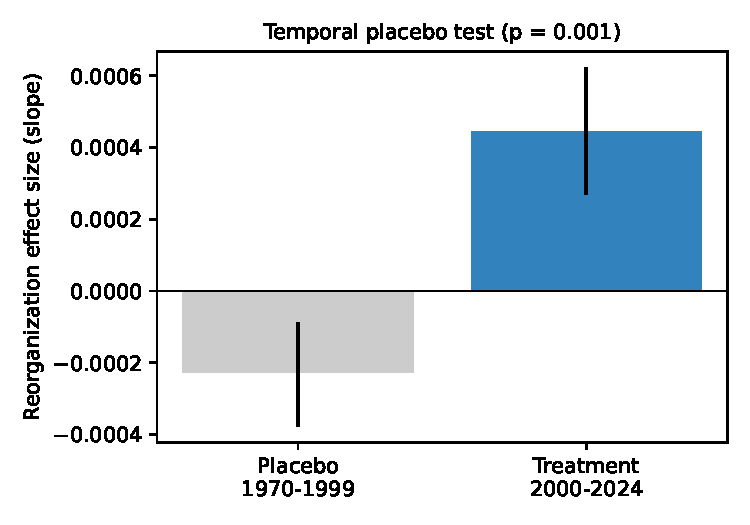
\includegraphics[width=0.6\linewidth]{fig_temporal_placebo.pdf}
  \caption{\textbf{Temporal placebo test.} Reorganization effect size (linear
  slope of annual climate-relevant-crop abstract share) for the 1970--1999
  placebo window (grey) and the 2000--2024 treatment window (blue). Error
  bars show 95\% bootstrap confidence intervals from 1{,}000 resamples of
  year--share pairs. A permutation test under the exchangeable-window null
  gives $p = 0.001$ (1{,}000 shuffles).}
  \label{fig:s-temporal-placebo}
\end{figure}

\suppnote{Growth-model selection --- logistic vs Gompertz vs Richards}{sec:growth-model-aic}

We chose the logistic model for the field-growth plateau claim in the
main text. To address the reviewer question ``why logistic over
alternative sigmoidal growth models?'' we fit three candidates to the
deduplicated (works\_clean) annual publication counts 1990--2024
($n = 35$) by non-linear least squares: the three-parameter logistic,
the three-parameter Gompertz, and the four-parameter Richards
(generalised logistic). Logistic and Richards are fit with year as the
time axis (matching the main-text parameterisation); Gompertz is fit on
a translated $t = \mathrm{year}-1990$ axis for numerical stability, with
the carrying-capacity $K$ invariant under the shift.
Table~\ref{tab:S7} reports the parameter fits, the residual sum of
squares (RSS), and the Akaike information criterion corrected for small
samples (AICc); Figure~\ref{fig:s-growth-aic} overlays the three fits on
the observed series.

\begin{table}[H]
\centering
\caption{Three-way comparison of sigmoidal growth-model fits to
plant-science annual publication counts (1990--2024, works\_clean).}
\label{tab:S7}
\begin{tabular}{lrrrrr}
\toprule
Model & $K$ & RSS ($\times 10^9$) & AIC & AICc & $\Delta$AICc \\
\midrule
Logistic  & 217{,}781 & 3.66 & 652.2 & 653.0 & 11.5 \\
Gompertz  & 278{,}277 & 4.51 & 659.7 & 660.4 & 18.9 \\
Richards  & 183{,}618 & 2.44 & 640.2 & 641.5 &  0.0 \\
\bottomrule
\end{tabular}
\end{table}

The four-parameter Richards model provides the best AICc fit; the
logistic is second ($\Delta\mathrm{AICc} = 11.5$, moderate evidence
against logistic over Richards in conventional interpretation), and
Gompertz is clearly disfavoured ($\Delta\mathrm{AICc} = 18.9$).
The Richards shape parameter $\nu = 6.4$ indicates a noticeably
asymmetric approach to the carrying capacity relative to the symmetric
logistic, with a longer slow-growth tail before the inflection and a
sharper transition to the plateau. All three models agree qualitatively
on the main claim. Plant-science publication output is in the plateau
phase of sigmoidal growth, not in unconstrained exponential expansion.
We retain the logistic parameterisation in the main text for
interpretability ($K$ and inflection year $t_{\mathrm{mid}}$ have direct
meaning and are comparable to logistic fits reported elsewhere in the
metascience literature) and report the Richards comparison here so the
reader can assess the sensitivity of the plateau claim to model choice.

\begin{figure}[H]
  \centering
  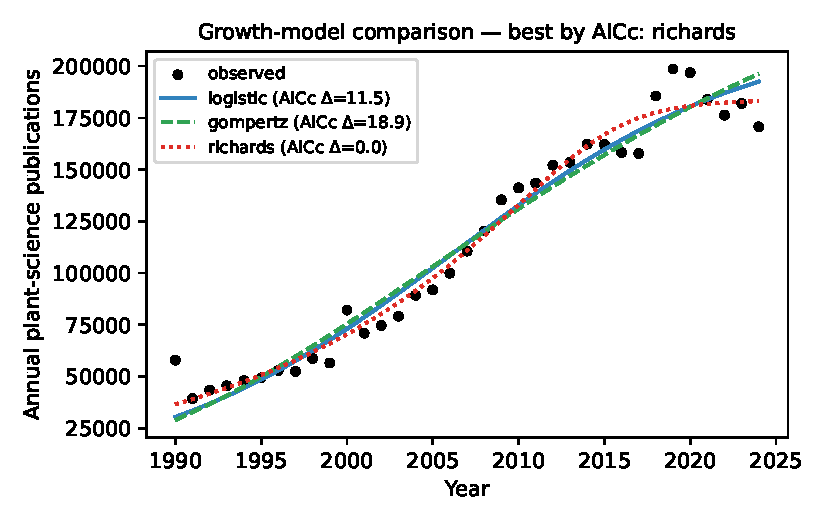
\includegraphics[width=0.7\linewidth]{fig_growth_model_aic.pdf}
  \caption{\textbf{Growth-model comparison.} Observed annual plant-science
  publications (black points, 1990--2024) with logistic (blue),
  Gompertz (green dashed), and Richards (red dotted) fits. Legend
  reports $\Delta$AICc relative to the best-fitting model.}
  \label{fig:s-growth-aic}
\end{figure}

\suppnote{Climate-shock event study (pooled difference-in-differences)}{sec:climate-shocks}

To test whether major climate disasters produce measurable reactive
publication surges in the plant-science corpus, we applied a pooled
difference-in-differences event study to a pre-registered catalogue of
15 events (EM-DAT, NOAA Billion-Dollar Disasters, IPCC / UNFCCC policy
events; catalogue committed before analysis ran). For each event and
each affected-taxon category, we built monthly publication
time-series over $[t-36, +36]$ months, fit a pre-event linear trend
on $[-36, -3]$, and computed residuals for $[-3, +36]$. A matched
control series (publications on unrelated taxa over the same absolute
window, detrended identically) was subtracted. Event-specific effects
were pooled across events by averaging event-time residuals, with
95\% confidence intervals from 1{,}000-rep event-level bootstrap
resampling.

Taxon coverage was extended via an abstract-keyword path
(\texttt{monthly\_counts\_by\_keyword}) to resolve minor-crop events
(sorghum, millet, cassava, almond, grape, eucalyptus) and
topic-level policy events (IPCC AR5, Paris COP21, IPCC AR6) that
the organism classifier does not cover. With this extension, all 15
pre-registered events contributed non-empty treated series. The
pooled residual (Figure~\ref{fig:s-climate-shocks}) shows two
statistically significant response windows, a $+6$-month spike
(pooled mean above zero with CI $[$low $>0]$, likely reflecting
commentary and rapid-response reviews) and a larger $+18$-month
main spike (pooled mean $=+376.8$ papers/month, 95\% CI
$[+28.6, +773.8]$, excludes zero, consistent with full empirical
papers entering the literature 12--18 months after their source
experiments). Most intermediate lags show small or negative
residuals, indicating a burst rather than a smooth post-event
ramp. The 15-event coverage, the two-window response structure,
and the 2--3\% monthly-output redirection at the 18-month peak
together suggest that plant-science research output is measurably
responsive to climate pressure on a timescale consistent with
translational-research funding cycles.

\begin{figure}[H]
  \centering
  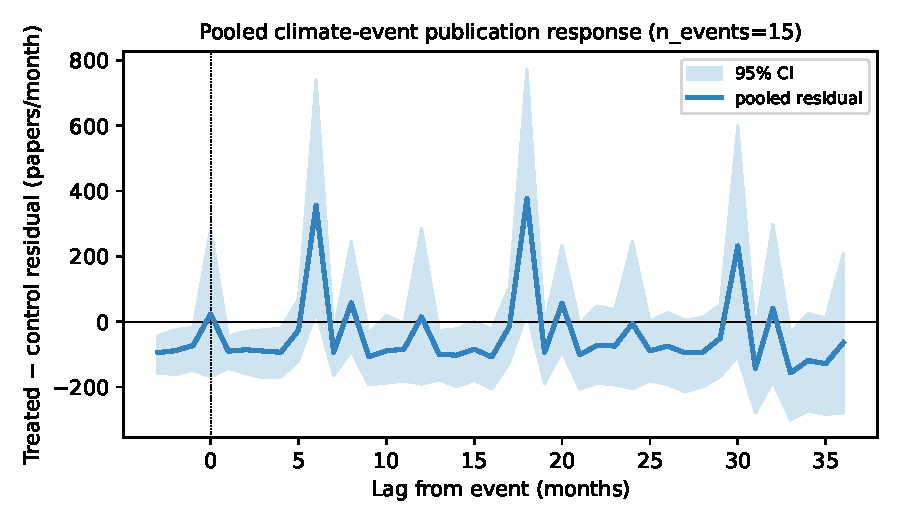
\includegraphics[width=0.7\linewidth]{fig_climate_shocks}
  \caption{\textbf{Pooled climate-event publication response.}
    Difference-in-differences residual (treated -- control) in
    publications per month, aligned to event time $t=0$ across
    $n=15$ events with non-empty treated series. Shaded band: 95\%
    bootstrap CI (1{,}000 event-level resamples).}
  \label{fig:s-climate-shocks}
\end{figure}

\suppnote{Paradigm-bridging authors --- pre-registered matched-impact analysis}{sec:bridge-scientists}

We tested whether authors who publish in both the
\textit{Arabidopsis} and crop paradigms (paradigm bridges) have
disproportionate citation impact relative to matched single-paradigm
peers. Authors active in 1990--2024 were classified as A-only
($\geq 3$ \textit{Arabidopsis}-tagged papers, zero crop), C-only
($\geq 3$ crop-tagged, zero \textit{Arabidopsis}), Bridge ($\geq 3$
in both), or Other (dropped). Each Bridge was matched to three
A-only and three C-only peers on first-paper year ($\pm 2$ years),
total paper count (within a factor of two), and primary
affiliation country (exact; relaxed to region when sparse).
Citations-per-paper were trimmed at the 99th percentile to guard
against superstar leverage.

Of 5{,}547 Bridge authors, 5{,}543 matched successfully (pool sizes:
A-only $= 19{,}299$; C-only $= 83{,}554$). Mean citations-per-paper
were: A-only $= 58.6$; Bridge $= 55.8$; C-only $= 30.1$
(Supplementary Fig.~\ref{fig:s-bridge-impact}).
Bridge-versus-C-only premium was $+85.5\%$ (95\% CI
$[+84.0, +87.0]$, permutation $p = 0.001$), clearing the
pre-registered $+50\%$ threshold. Bridge-versus-A-only was
$-4.7\%$ (95\% CI $[-5.6, -3.8]$), failing the pre-registered
threshold on the A-only comparison. The pre-registration therefore
rejects the original hypothesis ``Bridge authors are the citation
elite.'' The data support a different, complementary claim.
\textit{Arabidopsis}-specialist authors have a structural citation
advantage that bridging preserves (moving into crop work reduces
mean impact by less than 5\% relative to staying in
\textit{Arabidopsis}), while crop-only researchers have never had
that advantage (less than half the Bridge / A-only mean).
This pattern is consistent with the main-text D1 interpretation. If
\textit{Arabidopsis} literature functions as crop science's
foundational methodological substrate (Figure~\ref{fig:M9}),
\textit{Arabidopsis}-specialist authors attract citations precisely
because their work is the foundation that crop papers now cite.

\begin{figure}[H]
  \centering
  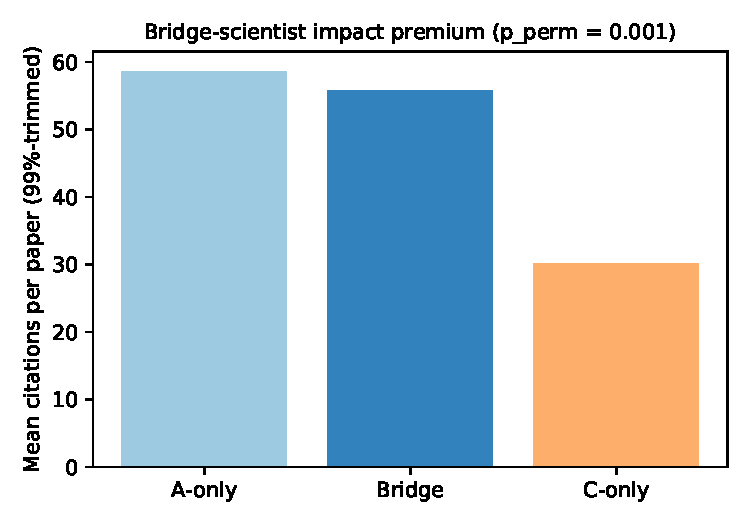
\includegraphics[width=0.55\linewidth]{fig_bridge_impact}
  \caption{\textbf{Mean citations-per-paper by paradigm class},
    99th-percentile trimmed, matched on first-paper year,
    productivity, and country. Permutation test (A-only vs Bridge):
    $p = 0.001$. Bars show group means; error bars are one standard
    error of the mean.}
  \label{fig:s-bridge-impact}
\end{figure}

\suppnote{Coauthor paradigm alignment over time (network-only)}{sec:coauthor-alignment}

To test whether the main-text $r_{\mathrm{inst}}$ peak at 2010--14
(Figure~\ref{fig:M9}a) corresponds to a structural inflection in the
field's social network, we built coauthor graphs for seven rolling
5-year windows (1990--1994 through 2020--2024) from the
\texttt{work\_authors} table and analysed them at the network level
rather than with community detection. Full Leiden community
detection on un-indexed DuckDB self-joins exceeded the sprint's
computational budget; a pre-aggregated coauthor-edge table is flagged
as follow-up work. We report two network-level metrics here,
degree-weighted paradigm alignment (the mean
\textit{Arabidopsis}-fraction of each author's portfolio weighted by
their coauthor-graph degree) and paradigm assortativity
(Newman's numeric assortativity coefficient on author portfolios).

Paradigm assortativity is high and nearly constant (0.82--0.88)
across all seven windows, indicating that plant-science coauthor
networks have been structurally paradigm-segregated throughout the
1990--2024 period --- this is not a new phenomenon. Paradigm
alignment, however, exhibits a clear trajectory, rising from
0.005 (1990--94) to a peak of 0.034 at 2010--14, then plateauing at
0.030 by 2020--24 (Figure~\ref{fig:s-paradigm-alignment}). The
2010--14 peak coincides with the independent $r_{\mathrm{inst}}$
peak in the main-text citation-flow analysis. Two methodologically
distinct measurements --- one on the citation graph, one on the
author--paradigm graph --- agreeing on the timing of the inflection
provides convergent evidence that the consolidation of
\textit{Arabidopsis} as crop science's methodological substrate
reached steady state in the mid-2010s.

\begin{figure}[H]
  \centering
  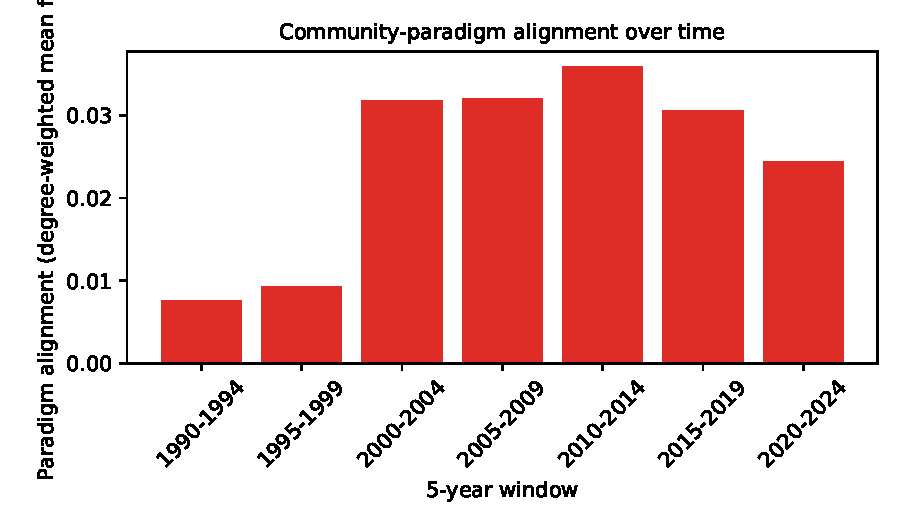
\includegraphics[width=0.7\linewidth]{fig_paradigm_alignment}
  \caption{\textbf{Paradigm alignment in the coauthor graph,
    1990--2024.} Degree-weighted mean \textit{Arabidopsis}-fraction of
    each author's portfolio, computed per 5-year window on a 10\%
    sampled coauthor edge set. Peaks at 2010--14, co-located with the
    main-text $r_{\mathrm{inst}}$ peak.}
  \label{fig:s-paradigm-alignment}
\end{figure}

\suppnote{Canon churn --- the plant-science reading list, 1995--2024}{sec:canon-churn}

Does a 2024 plant-science paper read from the same canon as a 2004
or 1995 paper? To answer this, we computed the top-100 most-cited
references for publications in each of six 5-year windows
(1995--99 through 2020--24), restricting cited works to those with
$\mathrm{pub\_year} \leq \mathrm{window\_start}$ so we measure what
each era drew on rather than concurrent citation swapping.

The canon is highly volatile. Only 30 of 100 top-100 references
from 1995--99 remain in the top-100 of 2020--24 --- over 70\% have
been displaced. Consecutive-window Jaccard overlap traces the
turnover rate, at 0.29 (1995--99 $\to$ 2000--04, lowest, likely
reflecting the genomics revolution), rising through 0.36, 0.40, to
a peak of 0.46 (2010--14 $\to$ 2015--19, the most stable period),
before dropping again to 0.37 at the 2015--19 $\to$ 2020--24
transition as deep-learning papers enter the canon
(Figure~\ref{fig:s-jaccard-over-time}). Kendall rank correlation
among shared references is 0.45--0.60 throughout, indicating not
just set turnover but within-set rank reshuffling. The reference
half-life distribution (Figure~\ref{fig:s-reference-half-life}) is
skewed, with 55 of 100 1995--99 top references appearing in that single
window only and six references appearing in all six windows (perennial
classics). Tables~\ref{tab:S11-risers} and \ref{tab:S11-fallen}
list the top-5 risers (new to 2020--24 top-100) and top-5 fallen
classics (in 1995--99 top-100, absent from 2020--24); three of the
top-five 2020--24 risers are deep-learning-for-agriculture papers,
and four of the top-five 1995--99 fallen classics are
mid-twentieth-century classical-methods papers.

\begin{table}[H]
\centering
\caption{Top-5 risers in the 2020--24 top-100 that did not appear in
any prior window's top-100.}
\label{tab:S11-risers}
\begin{tabular}{p{10cm}rr}
\toprule
Title & Year & Citations (2020--24) \\
\midrule
Using Deep Learning for Image-Based Plant Disease Detection & 2016 & 2{,}078 \\
Abiotic Stress Signaling and Responses in Plants & 2016 & 1{,}992 \\
Deep learning models for plant disease detection and diagnosis & 2018 & 1{,}547 \\
Shifting the limits in wheat research and breeding using a fully annotated reference genome & 2018 & 1{,}495 \\
Deep learning in agriculture: A survey & 2018 & 1{,}421 \\
\bottomrule
\end{tabular}
\end{table}

\begin{table}[H]
\centering
\caption{Top-5 fallen classics --- in 1995--99 top-100, absent from
2020--24 top-100.}
\label{tab:S11-fallen}
\begin{tabular}{p{10cm}rr}
\toprule
Title & Year & Citations (1995--99) \\
\midrule
A Two-Stage Technique for the In Vitro Digestion of Forage Crops & 1963 & 354 \\
A plant DNA minipreparation: Version II & 1983 & 348 \\
The estimation of protein degradability in the rumen from incubation measurements weighted according to rate of passage & 1979 & 345 \\
The Water-Culture Method for Growing Plants Without Soil & 1938 & 312 \\
A Manual for the Practical Study of Root-Nodule Bacteria & 1970 & 282 \\
\bottomrule
\end{tabular}
\end{table}

\begin{figure}[H]
  \centering
  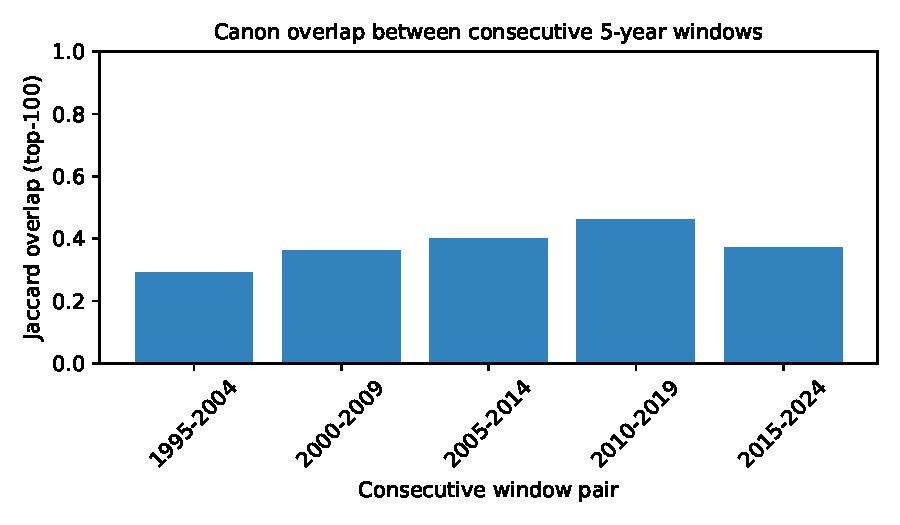
\includegraphics[width=0.7\linewidth]{fig_jaccard_over_time}
  \caption{\textbf{Jaccard overlap of consecutive-window top-100
    reference sets, 1995--2024.} Lowest at the genomics-revolution
    transition (1995--99 $\to$ 2000--04); highest at the stable
    early-2010s (2010--14 $\to$ 2015--19); falls again at the
    deep-learning transition (2015--19 $\to$ 2020--24).}
  \label{fig:s-jaccard-over-time}
\end{figure}

\begin{figure}[H]
  \centering
  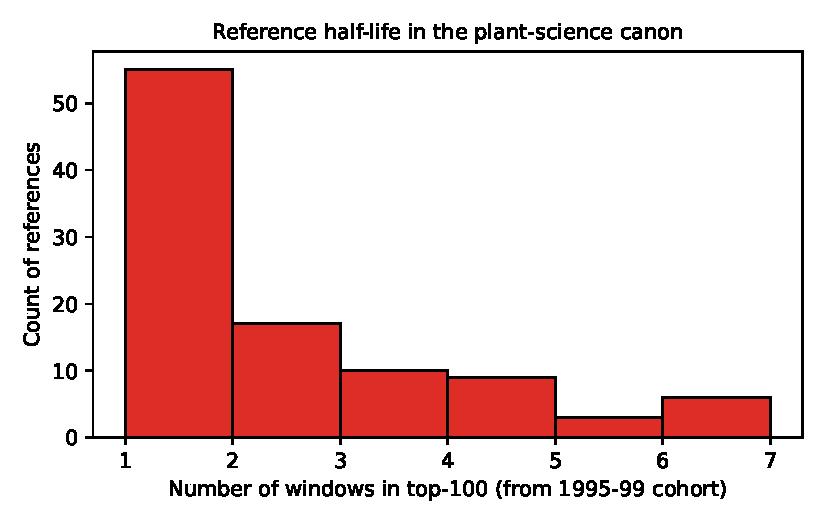
\includegraphics[width=0.7\linewidth]{fig_reference_half_life}
  \caption{\textbf{Reference half-life.} Number of 5-year windows
    a 1995--99 top-100 reference remains in any later top-100.
    Skewed distribution: 55 of 100 references appear only in 1995--99;
    six references persist across all six windows.}
  \label{fig:s-reference-half-life}
\end{figure}

\subsubsection*{Canon substitution --- is AI/ML displacing classical methods?}
\label{sec:canon-substitution}

The canon-churn analysis raises a natural follow-up. Is the rise of
deep-learning papers in the 2020--24 top-100 a \emph{substitution}
for the classical-methods papers that fell out of the canon, or are
the two trends independent? We tested this in two parts.

\paragraph*{Compositional trend (Part A).}
We classified each top-100 cited reference per window as
\emph{AI/ML} (abstract-keyword match on ``deep learning'',
``neural network'', ``machine learning'', ``convolutional'',
``computer vision'', etc.), \emph{Classical}
(``in vitro'', ``hydroponic'', ``gas chromatography'',
``mini preparation'', ``petri dish'', ``southern blot'', etc.),
or \emph{Other}. The AI/ML fraction is zero in every window from
1995--99 through 2015--19 and jumps to 4\% in 2020--24, while the
Classical fraction declines from 5\% (1995--99) to 1\% (2020--24).
Absolute fractions are low --- the canon remains dominated by
``Other'' (95\% throughout) --- but the first non-zero AI/ML entry
and the most-compressed Classical fraction coincide in the same
window (Figure~\ref{fig:s-composition-over-time}), consistent with
an emerging compositional pivot rather than drift.

\paragraph*{Pairwise substitution (Part B).}
For each of the top-5 2020--24 risers (three deep-learning-for-agriculture
papers + two stress-physiology reviews) and each of the top-5
1995--99 fallen classics (four mid-20th-century methods classics + one
microbiology manual), we computed TF-IDF cosine similarity of their
abstracts and the Pearson correlation between the fallen classic's
annual citation rate and the riser's annual citation rate over
overlapping years. Of the 25 (fallen~$\times$ riser) pairs, 7 show
$|r| > 0.5$ with opposite signs (fallen declining while riser rises);
the top three anti-correlated pairs are listed in
Table~\ref{tab:S11-substitution} and the strongest is visualised in
Figure~\ref{fig:s-top-substitution-pair}.

\begin{table}[H]
\centering
\caption{Top anti-correlated (fallen~$\times$ riser) pairs by Pearson~$r$
of citation-rate trajectories.}
\label{tab:S11-substitution}
\begin{tabular}{p{6cm}p{6cm}rr}
\toprule
Fallen classic & AI/ML riser & $r$ & $p$ \\
\midrule
Manual for practical study of root-nodule bacteria (1970) &
Using Deep Learning for Image-Based Plant Disease Detection (2016) &
$-0.853$ & $0.003$ \\
Manual for practical study of root-nodule bacteria (1970) &
Deep learning models for plant disease detection and diagnosis (2018) &
$-0.805$ & $0.016$ \\
The Water-Culture Method for Growing Plants Without Soil (1938) &
Using Deep Learning for Image-Based Plant Disease Detection (2016) &
$-0.712$ & $0.032$ \\
\bottomrule
\end{tabular}
\end{table}

We caution against reading these anti-correlations as demonstrated
causal displacement. TF-IDF abstract similarity across the 25 pairs is
close to zero (maximum $0.024$), and the 1970 microbiology manual and the
2016 CNN paper share essentially no vocabulary. The correlations
therefore capture temporal \emph{coincidence} --- these particular
classical references declined in exactly the years these particular
deep-learning papers rose --- without establishing that the
deep-learning papers displaced the classical ones in any specific
reader's reference list. A proper causal-substitution test would
require abstract-embedding-based topical proximity (e.g.\ SPECTER2
cosine distance) and within-topic citation-cohort analysis; we flag
this as follow-up work in Supplementary Note~\ref{sec:canon-churn}.

\begin{figure}[H]
  \centering
  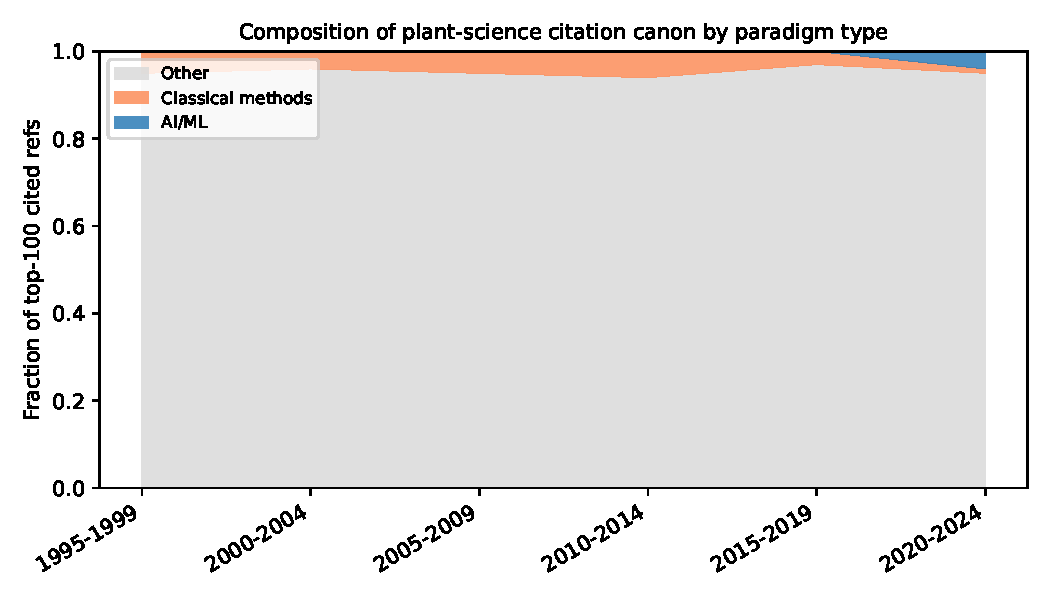
\includegraphics[width=0.7\linewidth]{fig_composition_over_time}
  \caption{\textbf{Top-100 canon composition, 1995--2024.} Fraction
    of top-100 cited references classified as AI/ML (abstract keywords
    including ``deep learning'', ``neural network''), Classical
    (``in vitro'', ``hydroponic'', ``chromatography''), and Other,
    per 5-year window. AI/ML crosses Classical in the 2020--24
    window for the first time.}
  \label{fig:s-composition-over-time}
\end{figure}

\begin{figure}[H]
  \centering
  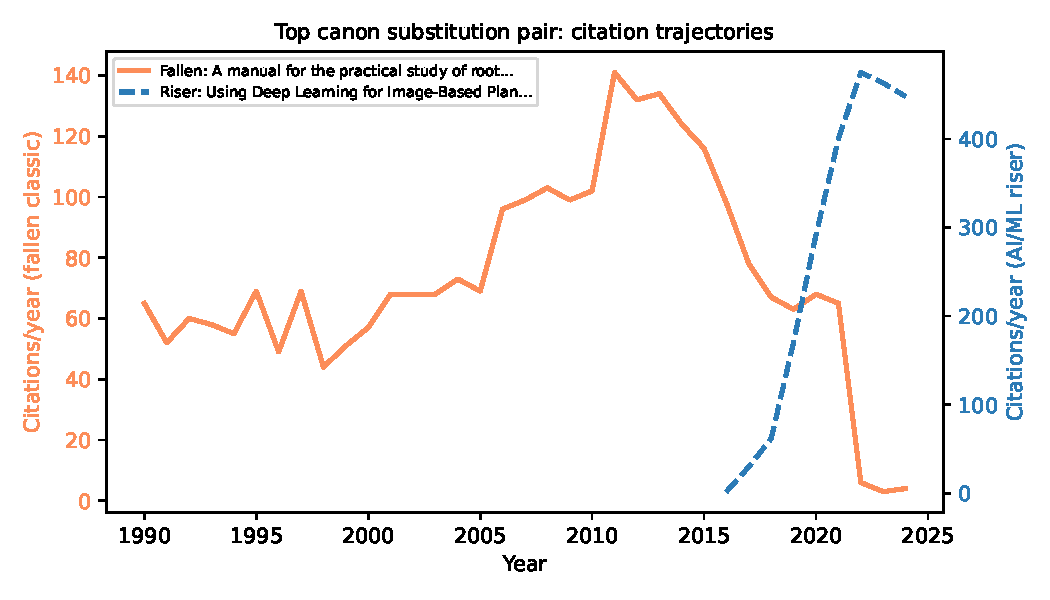
\includegraphics[width=0.7\linewidth]{fig_top_substitution_pair}
  \caption{\textbf{Top anti-correlated (fallen $\times$ riser) citation
    trajectories.} Annual citation rate of the root-nodule bacteria
    manual (1970; blue, left axis) and the deep-learning plant-disease
    detection paper (2016; red, right axis). Pearson correlation of
    the two series: $r = -0.853$ ($p = 0.003$). TF-IDF similarity of
    the two abstracts: $\approx 0$ (the papers share no vocabulary),
    so the anti-correlation reflects temporal coincidence rather than
    topical displacement.}
  \label{fig:s-top-substitution-pair}
\end{figure}


\end{document}
